% Simulation-informed revision: canonical pooling, mechanism diagnostics, and compound PPBRC neighbourhoods.
%%=====================================================================
%%  Cap-and-Trade Multi-Depot Vehicle Routing Problem (CT-MDVRP)
%%  Method: PPBRC
%%  Target journal: European Journal of Operational Research
%%  Compiled with uploaded Elsevier elsarticle template
%%=====================================================================
\documentclass[authoryear,final,3p,times]{elsarticle}

\usepackage{amssymb}
\usepackage{amsmath}
\usepackage{tikz}
\usetikzlibrary{arrows.meta,calc,positioning,fit,backgrounds}
\usepackage{graphicx}
\usepackage{float}
\usepackage{placeins}
\usepackage{booktabs}
\usepackage[ruled,vlined]{algorithm2e}
\usepackage{multirow}
\usepackage{amsthm}


\newtheorem{lemma}{Lemma}
\newtheorem{proposition}{Proposition}
\newtheorem{corollary}{Corollary}
\theoremstyle{definition}
\newtheorem{remark}{Remark}
\theoremstyle{plain}

\renewcommand{\topfraction}{0.9}
\renewcommand{\bottomfraction}{0.8}
\renewcommand{\textfraction}{0.05}
\renewcommand{\floatpagefraction}{0.8}

\allowdisplaybreaks


\begin{document}
\begin{frontmatter}

\title{Carbon-Price Coordination in the Cap-and-Trade Multi-Depot Vehicle
Routing Problem: A Matheuristic with Anytime Certification}

\author[label1]{Yang Zou}
\author[label2]{Yunqiang Yin\corref{cor1}}
\ead{yinyq@uestc.edu.cn}
\author[label3]{T.C.E. Cheng}
\cortext[cor1]{Corresponding author.}

\affiliation[label1]{organization={Yangtze Delta Region Institute (Huzhou),
  University of Electronic Science and Technology of China},
  city={Huzhou}, postcode={313001}, country={China}}
\affiliation[label2]{organization={School of Economics and Management,
  University of Electronic Science and Technology of China},
  city={Chengdu}, postcode={611731}, country={China}}
\affiliation[label3]{organization={Department of Logistics and Maritime Studies,
  The Hong Kong Polytechnic University},
  addressline={Hung Hom, Kowloon}, city={Hong Kong}, country={China}}

\begin{abstract}
Under a mandatory cap-and-trade scheme, fleet carbon emission is not an
\emph{ex post} indicator but an endogenous operational decision. This paper
introduces the Cap-and-Trade Multi-Depot Vehicle Routing Problem (CT-MDVRP),
in which several depots operate under a single shared corporate allowance and
load-dependent emissions enter the objective through a non-smooth market
settlement. We give a mixed-integer linear formulation with depot eligibility,
soft time windows, single-commodity payload flow, and an exact epigraph
representation of the buy--sell settlement, and we show that the settlement is
the only fleet-level term coupling routes across depots. Two structural
results follow. An exact regime decomposition splits the integer problem into
two side-constrained mixed-integer programmes and removes the kink without
approximation. Under a convex idealisation of the routing--emission frontier,
the cost-minimising emission obeys a three-regime law---permit-buying,
permit-neutral, and permit-selling---whose two thresholds are the emission
levels at which the marginal abatement cost equals the purchase and sale
prices, and whose neutral band widens with the buy--sell spread and collapses
to a carbon tax when the spread vanishes. This structure is the operating
principle of the proposed method rather than a description of it. We develop
CPCMAC, a carbon-price-coordinated matheuristic with anytime certification,
which represents the settlement by an internal carbon price inside the search
and coordinates that price at an outer level. The priced subproblem is exact
at either endpoint price whenever its solution lies on the correct side of the
allowance, so the coordination component commits its full budget to a single
price once a corner regime is detected. The inner solver is a strictly
feasible destroy--repair search with constant-time priced emission marginals
and a contextual bandit that selects the destroy operator from the internal
price, requiring no offline training. A Lagrangian $q$-route relaxation,
separable by depot and vehicle type, returns a valid anytime lower bound, so
every solution is reported with a certified optimality gap. The computational
study verifies CPCMAC against exact reference optima, isolates the
contribution of price coordination and of price-conditioned search, tests
whether the three-regime law survives the integrality of the routing
decisions, and quantifies the role of the buy--sell spread in setting the
permit-neutral band. The results characterise how regulatory stringency
reshapes cross-depot service boundaries and fleet consolidation.
\end{abstract}

\begin{keyword}
Transportation \sep Multi-depot vehicle routing \sep Cap-and-trade \sep
Matheuristic \sep Lagrangian relaxation
\end{keyword}

\end{frontmatter}

%%=====================================================================
\section{Introduction}
\label{sec:introduction}

The modern vehicle routing problem originates from cost-minimising fleet dispatch \citep{dantzig1959truck}, and environmental extensions now bring fuel use and carbon emission into the routing objective. Green road-freight studies show that emissions are affected not only by distance but also by vehicle load, speed, and sequencing decisions, and the Green Vehicle Routing Problem (GVRP) has become a standard operational-research paradigm for internalising these effects \citep{erdogan2012green,demir2014green,moghdani2021green}. This paper follows that emission-aware tradition but treats carbon as a market-settled operational cost rather than as a purely environmental performance indicator.

Conventional GVRP formulations nevertheless treat carbon emission either as a static exogenous penalty or as an \emph{ex post} performance measure. Neither treatment matches the institutional logic of a mandatory cap-and-trade scheme, in which operations are evaluated against a finite allowance and surplus or deficit emissions are settled through permit sales or purchases \citep{benjaafar2013carbon,hua2011managing}. Under a corporate allowance, the settlement cost is a convex piecewise-linear function of aggregate emission whose two slopes are the market purchase and sale prices, with a kink at the allowance. The cost-minimising fleet emission therefore ceases to be a downstream accounting artefact and becomes an endogenous decision determined jointly by spatial routing, payload distribution, and market conditions. The marginal cost of an additional unit of emission depends on the firm's position relative to its allowance, so the objective space of the routing problem is reshaped by the regulatory parameters themselves.

The multi-depot configuration compounds this difficulty. In the classical Multi-Depot Vehicle Routing Problem (MDVRP), customer-to-depot allocation and routing are intertwined, and fixing the allocation can decompose the problem into independent single-depot subproblems \citep{renaud1996tabu,cordeau1997vrp,montoyatorres2015literature}. A shared corporate allowance eliminates that decomposability: because the settlement is evaluated on the aggregate emission of the entire network, the marginal valuation of emission at one depot depends on the emissions produced at every other depot. A local perturbation at one depot can move the fleet across the allowance boundary and thereby alter the marginal carbon cost faced everywhere. Multi-depot green routing has been studied under pure emission-minimisation objectives, but the fleet-level economic interdependence induced by a market settlement has not been addressed. We close this gap by formalising the Cap-and-Trade Multi-Depot Vehicle Routing Problem (CT-MDVRP).

Existing algorithmic frameworks are ill-equipped for this coupling. Adaptive Large Neighbourhood Search (ALNS) is a dominant vehicle-routing metaheuristic, including for pollution-routing variants with nonlinear fuel evaluation \citep{ropke2006adaptive,demir2012alns}, and recent learning-augmented large-neighbourhood-search methods adapt operator selection or move generation from search-state information \citep{hottung2020neural,reijnen2024online,johnn2024graph}. These mechanisms select operators from generic spatial features, learned policies, or historical operator performance, and are therefore blind to the position of the fleet relative to the allowance, even though an identical perturbation carries a different economic value on either side of it. Two further obstacles are specific to the CT-MDVRP. First, evaluating the non-smooth settlement inside every neighbourhood move is expensive, and the sequence-dependent payload emission that drives it must itself be evaluated exactly. Second, the settlement is the only non-separable term of the objective, so a method that embeds it in each local evaluation pays a fleet-level price for a route-level decision. An effective framework must therefore separate the two levels rather than conflate them.

This observation motivates our approach. We show that the settlement admits a support-function representation over the buy--sell price interval, so that fixing an internal carbon price yields a routing problem whose carbon term is linear and whose kink has been removed. Coordinating that internal price at an outer level restores the fleet-level allowance logic exactly where it belongs, and the price that clears the allowance is precisely the threshold identified by the structural analysis. The resulting method, the Carbon-Price-Coordinated Matheuristic with Anytime Certification (CPCMAC), is thus derived from the structure of the problem rather than assembled from generic components. The contributions of the paper are threefold.

\begin{enumerate}
    \item \textbf{Formulation and structural characterisation.} We model the CT-MDVRP as a mixed-integer linear programme capturing load-dependent emission, depot eligibility, soft time windows, and the exact buy--sell epigraph, and we establish that the schedule and the payload flow are determined by the combinatorial decisions alone. We give an exact regime decomposition that removes the settlement kink on the integer problem at the cost of one side constraint per branch, and we prove that, under a convex idealisation of the routing--emission frontier, the optimal emission obeys a three-regime law whose thresholds are the price-anchored emission levels and whose permit-neutral band widens with the buy--sell spread, degenerating to a linear carbon tax when the spread vanishes.

    \item \textbf{A structure-derived matheuristic with a certified bound.} CPCMAC has three components. The coordination component prices the settlement internally, exploits the fact that the priced subproblem is an exact reformulation at either endpoint price whenever its solution lies on the correct side of the allowance, and otherwise locates the clearing price by a safeguarded bisection on the emission response, which is a valid supergradient of the concave dual. The inner solver is a strictly feasible destroy--repair search in which constant-time priced emission marginals follow from route labels and the destroy operator is selected by a discounted contextual bandit conditioned on the internal price, so that operator knowledge is amortised across the prices queried by the outer loop without any offline training. The certification component returns a valid anytime lower bound from a Lagrangian $q$-route relaxation that separates by depot and by vehicle type, so that every reported solution carries an optimality gap that depends on neither the bandit state nor the realised operator sequence.

    \item \textbf{Computational validation and managerial implications.} We verify CPCMAC against exact reference optima computed from the regime decomposition, compare it against a direct-settlement search under an identical budget with results stratified by regime, and isolate the contribution of price coordination and of price-conditioned search. We then test whether the three-regime law remains visible once routing decisions are integral, quantify how the buy--sell spread sets the permit-neutral band and the exact-compliance rate, and compare cap-and-trade against a carbon tax, a hard cap, and no regulation on identical instances. The results characterise how regulatory stringency reshapes cross-depot service boundaries and fleet consolidation.
\end{enumerate}

The remainder of this paper is organised as follows. Section~\ref{sec:literature_review} reviews the related literature. Section~\ref{sec:problem_formulation} presents the two-stage stochastic CBAR-MDVRP, and Section~\ref{sec:carbon_recourse} develops its price-polyhedral recourse structure. Section~\ref{sec:methodology} presents PPBRC, Section~\ref{sec:computational_experiments} describes the computational study, and Section~\ref{sec:conclusion} concludes.

%%=====================================================================
\section{Literature Review}
\label{sec:literature_review}

This section positions the CT-MDVRP and CPCMAC within the literature. Section~\ref{subsec:carbon_multi_depot} reviews carbon-regulated and multi-depot vehicle routing, focusing on the spatial and economic coupling induced by cap-and-trade mechanisms; Section~\ref{subsec:adaptive_learning_heuristics} reviews adaptive and learning-guided routing metaheuristics. Tables~\ref{tab:literature_taxonomy} and~\ref{tab:algorithmic_taxonomy} summarise the modelling and algorithmic positioning.

\subsection{Carbon-Regulated and Multi-Depot Routing}
\label{subsec:carbon_multi_depot}

Environmental imperatives have shifted vehicle routing models from distance- or time-centric optimisation to emission-aware distribution planning, with the Green Vehicle Routing Problem and green road-freight literature providing the paradigm for internalising these externalities \citep{erdogan2012green,demir2014green,moghdani2021green}. The Pollution-Routing Problem and related fuel-consumption models establish that fuel use and greenhouse gas emissions are not simple linear functions of travel distance but are jointly governed by vehicle payload, speed, and route sequencing \citep{bektas2011pollution,xiao2012development,demir2012alns}. Carbon-related routing costs must therefore be evaluated through sequence-dependent payload dynamics, which renders static distance-based approximations inadequate.

Building on these emission dynamics, a growing literature embeds carbon regulatory frameworks in operational models. Under a mandatory cap-and-trade scheme a firm operates subject to a finite corporate allowance: surplus permits may be sold, whereas deficits must be covered by market purchases, a structure widely used in supply-chain carbon-footprint models \citep{benjaafar2013carbon,hua2011managing}. Unlike a linear carbon tax, cap-and-trade therefore induces a non-smooth, piecewise-linear, regime-switching cost. \citet{fang2017reducing} and \citet{jharkharia2020vehicle} examined the economic implications of cap-and-trade for production-routing and order-picking problems, showing how market parameters alter the optimal operational trade-off. \citet{shen2018multi} considered carbon trading in a multi-depot open routing context. These studies quantify the economic impact of carbon trading through computational sensitivity analyses, but they do not characterise the allowance boundary analytically: the threshold at which the marginal cost of an emission perturbation changes discretely with the firm's carbon position remains unidentified, and with it the question of when the physical plan responds to the cap at all.

The difficulty compounds in multi-depot topologies. The MDVRP introduces a spatial-allocation layer, since assigning a customer to an alternative depot reshapes workloads, route lengths, and fleet activations \citep{renaud1996tabu,cordeau1997vrp,montoyatorres2015literature}; in green or operationally richer variants this flexibility operates as a decarbonisation or workload-balancing mechanism \citep{alinaghian2018multi,zhang2020multi,wen2022adaptive}. The interplay between multi-depot allocation and cap-and-trade regulation nevertheless remains unexplored. Reassigning a boundary customer across depots simultaneously alters local travel distances and downstream payloads, and because the settlement is executed at the aggregate corporate level, such a local reassignment propagates through the fleet-wide emission balance and can move the firm across a regime boundary. As Table~\ref{tab:literature_taxonomy} shows, existing studies treat multi-depot topologies, cap-and-trade settlements, load-dependent emissions, and soft time windows in isolation. The present study integrates them in a single formulation, derives the regime boundaries and the width of the permit-neutral band in closed form under a convex idealisation, and shows that these thresholds are computable as the emissions of two priced routing problems.

\begin{table}[!htbp]
\centering
\caption{Taxonomy of carbon-regulated and multi-depot vehicle routing studies.}
\label{tab:literature_taxonomy}
\footnotesize
\setlength{\tabcolsep}{5pt}
\renewcommand{\arraystretch}{1.2}
\begin{tabular}{@{}llclll@{}}
\toprule
Study & MD & TW & Carbon policy & Emission basis & Solution method \\
\midrule
\citet{bektas2011pollution}    & N & Hard & Tax / cost              & Load \& speed        & MILP (CPLEX) \\
\citet{demir2012alns}          & N & Hard & Tax / cost              & Load \& speed        & ALNS \\
\citet{fang2017reducing}       & N & --   & C\&T (regime-switch)    & Fuel cost$^{a}$      & Branch-and-cut \\
\citet{jharkharia2020vehicle}  & N & --   & C\&T (regime-switch)    & Dist.\ \& speed      & MILP (CPLEX) \\
\citet{shen2018multi}$^{b}$    & Y & Soft & C\&T (regime-switch)    & Fuel cost$^{a}$      & PSO $+$ tabu search \\
\citet{zhang2020multi}         & Y & --   & Minimisation            & Distance             & Ant colony \\
\citet{wen2022adaptive}        & Y & Hard & Minimisation            & Emission cost$^{a}$  & Improved ALNS \\
\textbf{This study}            & Y & Soft & C\&T (regime-switch)    & Exact load-dep.\     & CPCMAC \\
\bottomrule
\end{tabular}

\vspace{3pt}
\begin{minipage}{0.95\textwidth}
{\footnotesize \textit{Notes.} MD: multi-depot (Y/N). TW: time window.
$^{a}$ Formulations that include a fuel or carbon cost but do not explicitly model sequence-dependent payload dynamics.
$^{b}$ \citet{shen2018multi} models the \emph{open} routing variant, in which vehicles do not return to a depot.}
\end{minipage}
\end{table}

\subsection{Adaptive and Learning-Guided Routing Metaheuristics}
\label{subsec:adaptive_learning_heuristics}

The interaction of heterogeneous capacities, time windows, flexible depot assignments, and load-dependent emission dynamics places exact resolution beyond reach at operational scales. Adaptive Large Neighbourhood Search is a predominant metaheuristic for such problems: operating on a destroy--repair paradigm, it perturbs and reconstructs candidate solutions while preserving hard-constraint feasibility \citep{ropke2006adaptive}, and it has proved effective for the non-linear, sequence-dependent emission evaluations of the Pollution-Routing Problem \citep{demir2012alns}. Its standard operator-selection mechanism is nevertheless ill-matched to the CT-MDVRP. Reactive scoring updates operator probabilities from historical success frequencies and is therefore blind to the state of the incumbent, whereas in the CT-MDVRP the marginal utility of an operator is state-dependent: emission-oriented removals become valuable precisely when the effective carbon price is high, and cross-depot reassignments become valuable when depot flexibility is the cheapest abatement channel available.

Machine learning provides a basis for state-conditioned guidance \citep{bengio2021machine}. In routing, this integration follows three paradigms: end-to-end constructive policies that bypass classical search mechanics \citep{nazari2018reinforcement,kool2019attention}; learned step-wise perturbation policies that replace hand-crafted rules \citep{wu2022learning}; and learning agents embedded within an established search architecture, as in the deep-learning-assisted local search of \citet{zhao2021hybrid} and the reinforcement-learning meta-controller of \citet{qin2021rlhh}. Recent neural or reinforcement-learning large-neighbourhood-search variants further show how destroy--repair or operator-control decisions can be learned from the evolving search state \citep{hottung2020neural,reijnen2024online,johnn2024graph}. The last paradigm shows that a data-driven policy can serve as a high-level controller while the algorithmic substrate enforces feasibility. Its cost, however, is an offline training phase: the policy must be trained on an instance distribution and re-trained when the distribution or the objective changes. In the CT-MDVRP the objective changes with the internal carbon price at every step of the coordination loop, so a policy trained at one price is misspecified at another. This motivates an online, low-dimensional controller whose statistics are conditioned on the price and carried across the prices queried within a single run, rather than a network trained offline.

A complementary stream enhances neighbourhood search not by modifying operator selection but by adding a mathematical-programming component. Within the \emph{matheuristic} paradigm \citep{archetti2014matheuristics}, a heuristic navigates the solution space while an exact component periodically reoptimises the generated sub-structures; the canonical device for vehicle routing is set-partitioning post-optimisation over an archived route pool \citep{subramanian2013hybrid}, which frequently discovers configurations that the single-trajectory search never assembles. That device provides a primal improvement but no bound on the optimal value. The exact component of CPCMAC is placed on the dual side instead: the same internal price that renders the routing subproblem separable also yields, through a Lagrangian $q$-route relaxation, a valid lower bound on the CT-MDVRP, so that the method reports an optimality gap rather than only a possibly improved solution.

Finally, evaluating load-dependent emission remains a computational bottleneck irrespective of how operators are selected. Because payload propagates forward along a route, a local insertion or removal alters the load---and hence the fuel consumption---of all succeeding arcs, and recomputing the full trajectory for each candidate degrades the scalability of emission-aware neighbourhood search \citep{wen2022adaptive}. Table~\ref{tab:algorithmic_taxonomy} summarises how existing methods handle this evaluation.

\begin{table}[!htbp]
\centering
\caption{Algorithmic taxonomy of adaptive and learning-guided routing heuristics.}
\label{tab:algorithmic_taxonomy}
\footnotesize
\setlength{\tabcolsep}{6pt}
\renewcommand{\arraystretch}{1.25}
\resizebox{\textwidth}{!}{%
\begin{tabular}{@{}llll@{}}
\toprule
Study & Search paradigm & Guidance mechanism & Payload evaluation$^{a}$ \\
\midrule
\citet{ropke2006adaptive}       & ALNS (improvement)      & Reactive scoring                 & $\mathcal{O}(n)$ step-wise \\
\citet{demir2012alns}           & ALNS (improvement)      & Reactive scoring                 & $\mathcal{O}(n)$ step-wise \\
\citet{nazari2018reinforcement} & Constructive            & Actor--critic policy gradient    & Single-pass forward \\
\citet{kool2019attention}       & Constructive            & Attention-based policy rollout   & Single-pass forward \\
\citet{wu2022learning}          & Local search            & Self-attention policy gradient   & $\mathcal{O}(n)$ step-wise \\
\citet{zhao2021hybrid}          & Hybrid const.\ $+$ LS   & Learned policy $+$ standard LS   & $\mathcal{O}(n)$ step-wise \\
\citet{qin2021rlhh}             & Hyper-heuristic         & Policy-based meta-controller     & Sub-heuristic dependent \\
\citet{subramanian2013hybrid}   & ILS $+$ set partitioning & Reactive $+$ exact recombination & $\mathcal{O}(n)$ step-wise \\
\textbf{This study (CPCMAC)}    & Price-coordinated ALNS $+$ Lagrangian certification & Price-conditioned contextual bandit (online) $+$ anytime dual bound & Exact $\mathcal{O}(1)$ per-move label \\
\bottomrule
\end{tabular}}

\vspace{3pt}
\begin{minipage}{0.95\textwidth}
{\footnotesize \textit{Notes.} ``Reactive scoring'' refers to the dynamic adjustment of operator selection probabilities based on historical performance. ``Policy gradient/rollout'' indicates the training of neural models to output routing sequences or search actions.
$^{a}$ ``$\mathcal{O}(n)$ step-wise'' denotes element-wise recalculation of sequence-dependent downstream costs; ``single-pass forward'' denotes sequential route construction without subsequent local re-evaluation.}
\end{minipage}
\end{table}

Two gaps therefore emerge from Tables~\ref{tab:literature_taxonomy} and~\ref{tab:algorithmic_taxonomy}. On the modelling side, carbon-regulated routing studies capture cap-and-trade dynamics but bypass the spatial coupling of multi-depot operations, and none identifies the allowance thresholds at which the physical plan begins to respond to the cap. On the algorithmic side, no existing method combines an exact constant-time evaluation of load-dependent emission marginals, an operator controller conditioned on the prevailing carbon price and requiring no offline training, and a valid lower bound on the shared-allowance problem. The present study addresses both.

%%=====================================================================
\section{Problem Setting and Two-Stage Stochastic Formulation}
\label{sec:problem_formulation}

\subsection{Decision setting and timing}
\label{subsec:problem_description}

We consider a distribution firm that operates a set of depots
$\mathcal{D}$ under a centrally coordinated carbon-management programme.
The depots are operational units with separate carbon-performance accounts,
but they do not behave strategically: headquarters remains the single
decision maker and the legal counterparty in the external carbon market.
Before the demand of the next operating cycle is observed, headquarters
delegates a binding internal carbon budget to each depot.  The allocation is
used for responsibility accounting, performance evaluation, and the internal
assignment of external carbon costs; it is not a statutory allowance held by
the depot itself.

Once demand is realised, headquarters jointly determines the customer--depot
assignments and the vehicle routes.  The emissions of every route are charged
to the depot at which the route is rooted.  Demand uncertainty may therefore
leave some depot accounts in deficit and others in surplus relative to their
ex ante budgets.  The firm has two distinct classes of recourse.  First,
\emph{operational recourse} reallocates eligible boundary customers and
reconstructs vehicle routes, thereby changing physical emissions.  Second,
\emph{accounting recourse} transfers internal carbon credits through an
authorised depot-to-depot network and settles any residual account positions
through external purchases or sales.  Internal transfers incur directional
friction costs and are capacity limited, representing approval, accounting,
responsibility-adjustment, and internal-control restrictions.  External
transactions are executed centrally, but their costs or proceeds are assigned
to the depot accounts that generate the residual positions.

This distinction is material.  The ex ante budgets cannot be costlessly reset
after demand is observed; otherwise the first-stage allocation would be a
pure accounting convention.  Likewise, depot surpluses and deficits cannot be
netted outside the authorised internal-transfer network; otherwise the
transfer variables would be redundant.  The firm must consequently decide
where to place carbon responsibility before demand is known and, after demand
is observed, whether an imbalance should be corrected by moving service,
moving internal carbon credits, or trading externally.  We refer to the
resulting problem as the \emph{corporate carbon-budget allocation and recourse
multi-depot vehicle routing problem} (CBAR-MDVRP).

The decision sequence is as follows.  In the first stage, headquarters chooses
a budget vector $B=(B_d)_{d\in\mathcal D}$.  A demand scenario
$\omega\in\mathcal W$ is then realised.  In the second stage, the firm chooses
the customer assignments, vehicle routes, route payloads, depot emissions,
internal transfers, and external trades for that scenario.  Only $B$ is
non-anticipative; all routing and recourse decisions are scenario dependent.

\subsection{Network, uncertainty, and notation}
\label{subsec:notation}

The distribution system is defined on a directed graph
$\mathcal G=(\mathcal V,\mathcal A)$.  The customer set is $\mathcal C$ and the
depot set is $\mathcal D$.  Depot $d$ is represented by an origin node $o_d$
and a terminal node $r_d$.  The fleet is
$\mathcal K=\bigcup_{d\in\mathcal D}\mathcal K_d$, where $\mathcal K_d$ is the
set of vehicles stationed at depot $d$.  Vehicles may be grouped into classes
of identical units, $\mathcal K_d=\biguplus_{t\in\mathcal T_d}\mathcal K_{d,t}$;
$t(k)$ denotes the class of vehicle $k$.  Vehicles in the same class share
capacity $Q_k$, fixed dispatch cost $F_k$, maximum route duration $H_k$, and
empty- and full-load fuel rates $\rho_k^0$ and $\rho_k^Q$.  Heterogeneity is
retained as a modelling capability rather than as a separate contribution.

Each customer $i\in\mathcal C$ has a nonempty set of eligible depots
$\Omega_i\subseteq\mathcal D$.  Its home depot $h(i)\in\Omega_i$ is fixed,
and a customer with $|\Omega_i|\ge2$ is a boundary customer.  As in the
original formulation, eligibility may be generated by the distance-ratio rule
\begin{equation}
\Omega_i=\{h(i)\}\cup
\left\{d'\in\mathcal D\setminus\{h(i)\}:\;
\frac{d_{i,h(i)}}{d_{i,d'}}\ge\chi_\Omega\right\},
\qquad \chi_\Omega\in(0,1].
\label{eq:depot_flexibility}
\end{equation}
For vehicle $k$, let $d(k)$ denote its home depot,
$o_k=o_{d(k)}$, $r_k=r_{d(k)}$, and
$\mathcal C_k=\{i\in\mathcal C:d(k)\in\Omega_i\}$.  Its node and arc sets are
\begin{align*}
\mathcal V_k&=\mathcal C_k\cup\{o_k,r_k\},\\
\mathcal A_k&=\{(o_k,j):j\in\mathcal C_k\}
\cup\{(i,j):i,j\in\mathcal C_k,\ i\ne j\}
\cup\{(i,r_k):i\in\mathcal C_k\}.
\end{align*}
Every arc $(i,j)$ has distance $d_{ij}>0$, travel time $\tau_{ij}\ge0$, and
baseline operating cost $c_{ij}\ge0$.  Customer $i$ has service duration
$\sigma_i\ge0$.

Demand uncertainty is represented by a finite scenario set $\mathcal W$.
Scenario $\omega$ occurs with probability $\pi_\omega>0$, where
$\sum_{\omega\in\mathcal W}\pi_\omega=1$, and customer $i$ requires
$q_i^\omega>0$ units.  Customer locations, eligibility sets, arc data, fleet
parameters, and carbon-market prices do not vary across scenarios.  We assume
that every scenario is operationally feasible, in particular that each
customer can be served by at least one eligible vehicle and that the available
fleet can cover the realised demand.

The corporate carbon budget is $B^{\mathrm{corp}}$.  Headquarters chooses
$B_d$ for depot $d$, subject to lower and upper responsibility bounds
$\underline B_d$ and $\overline B_d$.  We assume
\begin{equation*}
\sum_{d\in\mathcal D}\underline B_d
\le B^{\mathrm{corp}}
\le\sum_{d\in\mathcal D}\overline B_d.
\end{equation*}
One unit of internal carbon credit covers one unit of route emission.

Internal transfers use the directed network
$\mathcal G^T=(\mathcal D,\mathcal A^T)$.  For
$a=(d,d')\in\mathcal A^T$, $\kappa_{dd'}\ge0$ is the unit transfer friction
and $\overline T_{dd'}\ge0$ is the transfer capacity.  Define the outgoing and
incoming transfer-arc sets
\begin{equation*}
\delta_T^+(d)=\{(d,d')\in\mathcal A^T\},
\qquad
\delta_T^-(d)=\{(d',d)\in\mathcal A^T\}.
\end{equation*}
Residual deficits are purchased externally at $p^{\mathrm{buy}}$, and residual
surpluses are sold at $p^{\mathrm{sell}}$, with
\begin{equation}
p^{\mathrm{buy}}>p^{\mathrm{sell}}\ge0.
\label{eq:market_spread}
\end{equation}
The strict spread rules out simultaneous purchase and sale as an optimal
accounting action and prevents external-market arbitrage.

Table~\ref{tab:main_notation} summarises the main notation introduced by the
reformulation.

\begin{table}[!htbp]
\centering
\caption{Main notation for the two-stage carbon-budget model.}
\label{tab:main_notation}
\footnotesize
\renewcommand{\arraystretch}{1.15}
\begin{tabular}{@{}lp{0.76\textwidth}@{}}
\toprule
Symbol & Meaning \\
\midrule
$\mathcal W,\pi_\omega$ & Demand scenarios and their probabilities. \\
$q_i^\omega$ & Demand of customer $i$ in scenario $\omega$. \\
$B^{\mathrm{corp}}$ & Corporate carbon budget available before demand is observed. \\
$B_d$ & First-stage internal carbon budget delegated to depot $d$. \\
$\mathcal G^T=(\mathcal D,\mathcal A^T)$ & Directed internal carbon-credit transfer network. \\
$\kappa_{dd'},\overline T_{dd'}$ & Unit friction and capacity of transfer arc $(d,d')$. \\
$p^{\mathrm{buy}},p^{\mathrm{sell}}$ & External purchase and sale prices. \\
$E_d^\omega$ & Route emission charged to depot $d$ in scenario $\omega$. \\
$t_{dd'}^\omega$ & Internal credits transferred from depot $d$ to depot $d'$ in scenario $\omega$. \\
$b_d^\omega,s_d^\omega$ & External purchase and sale assigned to depot $d$ in scenario $\omega$. \\
\bottomrule
\end{tabular}
\end{table}

\begin{table}[!htbp]
\centering
\caption{Decision variables.}
\label{tab:decision_variables}
\footnotesize
\renewcommand{\arraystretch}{1.15}
\begin{tabular}{@{}lp{0.76\textwidth}@{}}
\toprule
Variable & Meaning \\
\midrule
$B_d$ & First-stage carbon budget delegated to depot $d$; common to all scenarios. \\
$y_{id}^\omega$ & One if customer $i$ is assigned to depot $d$ in scenario $\omega$. \\
$z_i^{k\omega}$ & One if vehicle $k$ serves customer $i$ in scenario $\omega$. \\
$x_{ij}^{k\omega}$ & One if vehicle $k$ traverses arc $(i,j)$ in scenario $\omega$. \\
$a_k^\omega$ & One if vehicle $k$ is dispatched in scenario $\omega$. \\
$f_{ij}^{k\omega}$ & Payload carried by vehicle $k$ on arc $(i,j)$ in scenario $\omega$. \\
$E_d^\omega$ & Emission of routes rooted at depot $d$ in scenario $\omega$. \\
$t_{dd'}^\omega$ & Internal carbon credit transferred from $d$ to $d'$ in scenario $\omega$. \\
$b_d^\omega,s_d^\omega$ & External purchase and sale assigned to depot $d$ in scenario $\omega$. \\
\bottomrule
\end{tabular}
\end{table}

\subsection{Deterministic-equivalent mixed-integer formulation}
\label{subsec:mathematical_formulation}

The first-stage variable is $B_d\ge0$.  For every scenario $\omega$, the
binary variables are $y_{id}^\omega$ (customer--depot assignment),
$z_i^{k\omega}$ (vehicle service), $x_{ij}^{k\omega}$ (arc use), and
$a_k^\omega$ (vehicle dispatch).  The nonnegative continuous variables are
$f_{ij}^{k\omega}$ (payload), $E_d^\omega$ (depot emission),
$t_{dd'}^\omega$ (internal transfer), $b_d^\omega$ (external purchase), and
$s_d^\omega$ (external sale).

The deterministic equivalent is
\begin{align}
\min\quad Z={}&
\sum_{\omega\in\mathcal W}\pi_\omega\Bigg[
\sum_{k\in\mathcal K}F_k a_k^\omega
+\sum_{k\in\mathcal K}\sum_{(i,j)\in\mathcal A_k}
 c_{ij}x_{ij}^{k\omega}
\notag\\[-1mm]
&\hspace{29mm}
+\sum_{(d,d')\in\mathcal A^T}\kappa_{dd'}t_{dd'}^\omega
+p^{\mathrm{buy}}\sum_{d\in\mathcal D}b_d^\omega
-p^{\mathrm{sell}}\sum_{d\in\mathcal D}s_d^\omega
\Bigg]
\label{eq:obj}
\end{align}
subject to the first-stage budget constraints
\begin{align}
&\sum_{d\in\mathcal D}B_d=B^{\mathrm{corp}},
\label{eq:budget_total}\\
&\underline B_d\le B_d\le\overline B_d,
&&\forall d\in\mathcal D,
\label{eq:budget_bounds}
\end{align}
and, for every $\omega\in\mathcal W$, the routing constraints
\begin{align}
&\sum_{d\in\Omega_i}y_{id}^\omega=1,
&&\forall i\in\mathcal C,
\label{eq:c1}\\
&\sum_{k\in\mathcal K_d}z_i^{k\omega}=y_{id}^\omega,
&&\forall i\in\mathcal C,\ \forall d\in\Omega_i,
\label{eq:c2}\\
&z_i^{k\omega}\le a_k^\omega,
&&\forall k\in\mathcal K,\ \forall i\in\mathcal C_k,
\label{eq:c3}\\
&\sum_{i\in\mathcal C_k}z_i^{k\omega}\ge a_k^\omega,
&&\forall k\in\mathcal K,
\label{eq:c4}\\
&\sum_{j\in\mathcal C_k}x_{o_kj}^{k\omega}=a_k^\omega,
\qquad
\sum_{i\in\mathcal C_k}x_{ir_k}^{k\omega}=a_k^\omega,
&&\forall k\in\mathcal K,
\label{eq:c56}\\
&\sum_{j\in\mathcal C_k\cup\{r_k\}\setminus\{i\}}
 x_{ij}^{k\omega}=z_i^{k\omega},
&&\forall k\in\mathcal K,\ \forall i\in\mathcal C_k,
\label{eq:c7}\\
&\sum_{j\in\mathcal C_k\cup\{o_k\}\setminus\{i\}}
 x_{ji}^{k\omega}=z_i^{k\omega},
&&\forall k\in\mathcal K,\ \forall i\in\mathcal C_k,
\label{eq:c78}\\
&\sum_{(i,j)\in\mathcal A_k}\tau_{ij}x_{ij}^{k\omega}
 +\sum_{i\in\mathcal C_k}\sigma_i z_i^{k\omega}
 \le H_k a_k^\omega,
&&\forall k\in\mathcal K,
\label{eq:c12}
\end{align}
together with the single-commodity payload-flow constraints
\begin{align}
&\sum_{j\in\mathcal C_k}f_{o_kj}^{k\omega}
 =\sum_{i\in\mathcal C_k}q_i^\omega z_i^{k\omega},
&&\forall k\in\mathcal K,
\label{eq:c16}\\
&\sum_{j\in\mathcal C_k\cup\{o_k\}\setminus\{i\}}
 f_{ji}^{k\omega}
 -\sum_{j\in\mathcal C_k\cup\{r_k\}\setminus\{i\}}
 f_{ij}^{k\omega}
 =q_i^\omega z_i^{k\omega},
&&\forall k\in\mathcal K,\ \forall i\in\mathcal C_k,
\label{eq:c17}\\
&0\le f_{ij}^{k\omega}\le Q_k x_{ij}^{k\omega},
&&\forall k\in\mathcal K,\ \forall(i,j)\in\mathcal A_k,
\label{eq:c19a}\\
&f_{ir_k}^{k\omega}=0,
&&\forall k\in\mathcal K,\ \forall i\in\mathcal C_k.
\label{eq:c19b}
\end{align}
Because every $q_i^\omega$ is strictly positive, the payload-flow balance
excludes a customer subtour disconnected from the vehicle origin: summing
\eqref{eq:c17} over such a subtour would give zero net boundary flow but a
strictly positive total demand.

The load-dependent emission charged to depot $d$ is
\begin{align}
E_d^\omega={}&
\sum_{k\in\mathcal K_d}\sum_{(i,j)\in\mathcal A_k}
\theta d_{ij}\left[
\rho_k^0x_{ij}^{k\omega}
+\frac{\rho_k^Q-\rho_k^0}{Q_k}f_{ij}^{k\omega}
\right],
&&\forall d\in\mathcal D,
\label{eq:c20}
\end{align}
where $\theta>0$ converts fuel use into carbon emission and
$\rho_k^Q\ge\rho_k^0\ge0$.  The first term prices empty-vehicle distance,
whereas the second term captures the additional effect of the payload carried
on each arc.  Hence customer sequencing affects emissions even when route
distance is unchanged.

Internal transfers and depot carbon accounts satisfy
\begin{align}
&0\le t_{dd'}^\omega\le\overline T_{dd'},
&&\forall(d,d')\in\mathcal A^T,
\label{eq:transfer_capacity}\\
&B_d
+\sum_{(h,d)\in\delta_T^-(d)}t_{hd}^\omega
+b_d^\omega
=E_d^\omega
+\sum_{(d,h)\in\delta_T^+(d)}t_{dh}^\omega
+s_d^\omega,
&&\forall d\in\mathcal D.
\label{eq:account_balance}
\end{align}
The left-hand side of \eqref{eq:account_balance} is the carbon credit available
to depot $d$: its ex ante budget, incoming internal transfers, and external
purchases.  The right-hand side is its use of credit: route emissions,
outgoing transfers, and external sales.  The account equation is the only
constraint that directly connects the first-stage allocation to the
scenario-wise physical and financial recourse decisions.

The variable domains are
\begin{align}
&B_d\ge0,
&&\forall d\in\mathcal D,
\notag\\
&E_d^\omega,b_d^\omega,s_d^\omega\ge0,
&&\forall d\in\mathcal D,\ \forall\omega\in\mathcal W,
\notag\\
&x_{ij}^{k\omega},y_{id}^\omega,z_i^{k\omega},a_k^\omega\in\{0,1\},
&&\text{for all applicable }i,j,k,d,\omega,
\notag\\
&f_{ij}^{k\omega}\ge0,
\qquad
t_{dd'}^\omega\ge0,
&&\forall\omega\in\mathcal W,\ \forall k,\ (i,j)\in\mathcal A_k,\ (d,d')\in\mathcal A^T.
\label{eq:c_domain}
\end{align}
All second-stage constraints above are imposed for every
$\omega\in\mathcal W$; the scenario quantifier is suppressed after the first
line of each block to improve readability.

The objective \eqref{eq:obj} is measured in monetary units.  Its first two
terms are dispatch and travel costs, the third is the internal organisational
cost of reallocating carbon responsibility, and the last two terms are the
cost and revenue assigned to depot accounts from external trading.  Since
$p^{\mathrm{buy}}>p^{\mathrm{sell}}$, simultaneous external purchase and sale
at one depot cannot be optimal: reducing both variables by their smaller value
preserves \eqref{eq:account_balance} and strictly reduces the objective by the
buy--sell spread.  No additional binary market-status variable is required.

\paragraph{Scenario-wise combinatorial core.}
\label{subsec:reduction}

\begin{corollary}[Scenario-wise combinatorial core]
\label{cor:core}
Fix a scenario $\omega$ and a feasible binary routing plan
$(x^\omega,y^\omega,z^\omega,a^\omega)$.  Along each used route, the payload on
an arc is uniquely equal to the sum of the demands of the customers that
remain to be served.  Consequently the route duration and every depot emission
$E_d^\omega$ are uniquely determined by the customer assignments, route
partition, and customer sequences.  For a fixed first-stage budget $B$, the
remaining carbon-account contribution is the optimal value of the linear
recourse problem defined in Section~\ref{sec:carbon_recourse}.
\end{corollary}

\begin{proof}
Starting from the zero payload on the terminal arc, equations
\eqref{eq:c17}--\eqref{eq:c19b} determine the payloads backwards along each
route as suffix demands; \eqref{eq:c16} is then satisfied at the origin.
Substitution in \eqref{eq:c20} determines depot emissions.  Route duration is
the sum appearing in \eqref{eq:c12}.  Once $B$ and $E^\omega$ are fixed, only
the internal-transfer and external-trading variables remain in the carbon
accounts, and their minimum cost is the recourse value introduced below.
\end{proof}

\paragraph{Valid inequalities and symmetry breaking.}
\label{subsec:strengthening}

The scenario-wise arc-load inequalities
\begin{align}
&f_{ij}^{k\omega}\ge q_j^\omega x_{ij}^{k\omega},
&&\forall k\in\mathcal K,\ \forall(i,j)\in\mathcal A_k:\ j\in\mathcal C_k,
\label{eq:vi1}\\
&f_{ij}^{k\omega}\le(Q_k-q_i^\omega)x_{ij}^{k\omega},
&&\forall k\in\mathcal K,\ \forall(i,j)\in\mathcal A_k:\ i\in\mathcal C_k,
\label{eq:vi2}
\end{align}
strengthen the linear relaxation.  The first requires the payload entering
customer $j$ to include its demand; the second recognises that the demand of
customer $i$ has been delivered before an outgoing arc is traversed.  For
consecutive identical vehicles $k<k'$ in the same depot and class, the
scenario-wise ordering
\begin{equation}
a_k^\omega\ge a_{k'}^\omega,
\qquad
\forall d\in\mathcal D,\ \forall t\in\mathcal T_d,\ \forall\omega\in\mathcal W,
\quad k<k'\text{ consecutive in }\mathcal K_{d,t}.
\label{eq:vi3}
\end{equation}
removes dispatch-index symmetry without excluding all representatives of any
physical solution.

\subsection{Value-function form and institutional special cases}
\label{subsec:model_interpretation}

Let $\mathcal X(q^\omega)$ denote the feasible set of the scenario routing and
payload variables defined by \eqref{eq:c1}--\eqref{eq:c20}.  Let
$C_{\mathrm{op}}(S^\omega)$ be the dispatch and travel cost of a routing plan
$S^\omega\in\mathcal X(q^\omega)$, and let
$E(S^\omega)=(E_d(S^\omega))_{d\in\mathcal D}$.  The extensive-form model can
be written compactly as
\begin{equation}
\min_{B\in\mathcal B}
\sum_{\omega\in\mathcal W}\pi_\omega
\min_{S^\omega\in\mathcal X(q^\omega)}
\left\{
C_{\mathrm{op}}(S^\omega)
+\Psi_{\overline T}\bigl(E(S^\omega)-B\bigr)
\right\},
\label{eq:two_stage_value_form}
\end{equation}
where
\begin{equation*}
\mathcal B=\left\{B:
\sum_{d\in\mathcal D}B_d=B^{\mathrm{corp}},\quad
\underline B_d\le B_d\le\overline B_d\right\},
\end{equation*}
and $\Psi_{\overline T}$ is the network-constrained carbon-recourse value
function developed in Section~\ref{sec:carbon_recourse}.

Three institutional regimes are nested in the formulation.  Setting all
transfer capacities to zero gives independent depot accounts.  Positive
frictions and finite capacities give the network-constrained regime studied in
this paper.  If the transfer network is strongly connected, all transfer
frictions are zero, and capacities are sufficiently large never to bind, the
accounts can be rebalanced without friction and the model collapses to a fully
pooled corporate account.

The last regime also identifies a degeneracy.  Under frictionless uncapacitated
pooling, only the sum $\sum_dB_d=B^{\mathrm{corp}}$ affects recourse, so the
distribution of the first-stage budget may be non-unique and economically
irrelevant.  The allocation can likewise lose value when
$p^{\mathrm{buy}}=p^{\mathrm{sell}}$, or when every depot is always on the same
side of its budget so that no cross-depot netting opportunity arises.  The
first-stage decision is therefore economically active only when demand and
emission responsibilities are heterogeneous across depots and scenarios and
when internal transfers or external transactions are genuinely frictional.
These cases are institutional benchmarks rather than the default setting of
the model.

%%=====================================================================
\section{Carbon-Recourse Value and Price-Polyhedral Structure}
\label{sec:carbon_recourse}
\label{subsec:structural}

This section isolates the accounting recourse that remains after a scenario
routing plan has fixed the depot emissions.  The resulting value function is
an exact component of the mixed-integer model, requires no convexification of
the routing decisions, and provides the marginal carbon signals used by the
subsequent solution method.  Convexity claims in this section concern the
continuous recourse function for fixed routing emissions; they do not imply
that the complete two-stage stochastic routing problem is convex.

\subsection{Carbon-recourse value function}
\label{subsec:recourse_value}

Suppress the scenario superscript and define the depot net-deficit vector
\begin{equation}
g_d=E_d-B_d,
\qquad d\in\mathcal D.
\label{eq:net_deficit}
\end{equation}
A positive $g_d$ is a deficit and a negative $g_d$ is a surplus.  For fixed
$g$, the minimum carbon-account recourse cost is
\begin{align}
\Psi_{\overline T}(g)=
\min_{t,b,s}\quad&
\sum_{(d,d')\in\mathcal A^T}\kappa_{dd'}t_{dd'}
+p^{\mathrm{buy}}\sum_{d\in\mathcal D}b_d
-p^{\mathrm{sell}}\sum_{d\in\mathcal D}s_d
\label{eq:recourse_primal}\\
\text{s.t.}\quad&
 b_d+\sum_{(h,d)\in\delta_T^-(d)}t_{hd}
 -\sum_{(d,h)\in\delta_T^+(d)}t_{dh}-s_d=g_d,
&&\forall d\in\mathcal D,
\label{eq:recourse_balance}\\
&0\le t_{dd'}\le\overline T_{dd'},
&&\forall(d,d')\in\mathcal A^T,
\label{eq:recourse_capacity}\\
&b_d,s_d\ge0,
&&\forall d\in\mathcal D.
\label{eq:recourse_domain}
\end{align}

\begin{proposition}[Complete recourse and minimum-cost-flow structure]
\label{prop:recourse_flow}
For every $g\in\mathbb R^{|\mathcal D|}$, problem
\eqref{eq:recourse_primal}--\eqref{eq:recourse_domain} is feasible and has a
finite optimum.  It is a capacitated minimum-cost transshipment problem on the
internal transfer network augmented by an external-market node.
\end{proposition}

\begin{proof}
Feasibility follows by setting $t=0$, $b_d=[g_d]_+$, and
$s_d=[-g_d]_+$, where $[u]_+=\max\{u,0\}$.  To obtain the network
interpretation, add an external-market node.  A purchase is an arc from the
market node to depot $d$ with unit cost $p^{\mathrm{buy}}$, a sale is an arc
from depot $d$ to the market node with unit cost $-p^{\mathrm{sell}}$, and an
internal arc $(d,d')$ has cost $\kappa_{dd'}$ and capacity
$\overline T_{dd'}$.  The depot imbalances are $g$.  Internal cycles have
nonnegative cost, and every cycle that purchases externally and later sells
externally has cost at least
$p^{\mathrm{buy}}-p^{\mathrm{sell}}>0$.  Hence no negative-cost cycle can
create unbounded arbitrage, and the feasible transshipment problem has a
finite optimum.
\end{proof}

\begin{lemma}[No simultaneous external purchase and sale]
\label{lem:no_simultaneous_trade}
At an optimal solution of \eqref{eq:recourse_primal}, a depot cannot satisfy
$b_d>0$ and $s_d>0$ simultaneously.
\end{lemma}

\begin{proof}
If both variables are positive, decrease them by
$\varepsilon=\min\{b_d,s_d\}>0$.  The balance constraint is unchanged, whereas
the objective decreases by
$(p^{\mathrm{buy}}-p^{\mathrm{sell}})\varepsilon>0$.
\end{proof}

\subsection{Dual representation and the extended price polyhedron}
\label{subsec:price_polyhedron}

Associate a free multiplier $\lambda_d$ with the balance equation of depot
$d$ and a nonnegative multiplier $\mu_{dd'}$ with the upper bound on transfer
arc $(d,d')$.  The dual of \eqref{eq:recourse_primal} is
\begin{align}
\Psi_{\overline T}(g)=
\max_{\lambda,\mu}\quad&
\sum_{d\in\mathcal D}\lambda_d g_d
-\sum_{(d,d')\in\mathcal A^T}
 \overline T_{dd'}\mu_{dd'}
\label{eq:recourse_dual}\\
\text{s.t.}\quad&
p^{\mathrm{sell}}\le\lambda_d\le p^{\mathrm{buy}},
&&\forall d\in\mathcal D,
\label{eq:dual_price_bounds}\\
&\lambda_{d'}-\lambda_d-\mu_{dd'}\le\kappa_{dd'},
&&\forall(d,d')\in\mathcal A^T,
\label{eq:dual_transfer_arbitrage}\\
&\mu_{dd'}\ge0,
&&\forall(d,d')\in\mathcal A^T.
\label{eq:dual_mu_domain}
\end{align}
Define the extended price polyhedron
\begin{equation}
\widetilde\Lambda=
\left\{(\lambda,\mu):
\eqref{eq:dual_price_bounds}--\eqref{eq:dual_mu_domain}\right\}.
\label{eq:extended_price_polyhedron}
\end{equation}
The variable $\lambda_d$ is the marginal cost of an additional unit of
emission at depot $d$, equivalently the marginal saving from one additional
unit of budget at that depot while the routing emissions are fixed.  The
external market bounds this value between its sale and purchase prices.  The
arc inequality prevents a price difference from exceeding the cost of moving
one unit of internal credit, unless the transfer capacity is congested and
therefore carries a positive multiplier $\mu_{dd'}$.

\begin{proposition}[Price-polyhedral dual representation]
\label{prop:price_polyhedron}
For every $g$, strong linear-programming duality gives
\begin{equation}
\Psi_{\overline T}(g)=
\max_{(\lambda,\mu)\in\widetilde\Lambda}
\left\{
\lambda^\top g-\sum_{(d,d')\in\mathcal A^T}
\overline T_{dd'}\mu_{dd'}
\right\}.
\label{eq:extended_support_representation}
\end{equation}
If the model omits transfer capacities (or one restricts attention to a
region in which they are known not to bind), the capacity multipliers can be
omitted and
\begin{equation}
\Psi_\infty(g)=\max_{\lambda\in\Lambda}\lambda^\top g,
\label{eq:price_support_representation}
\end{equation}
where
\begin{equation}
\Lambda=
\left\{\lambda\in\mathbb R^{|\mathcal D|}:
 p^{\mathrm{sell}}\le\lambda_d\le p^{\mathrm{buy}},\quad
 \lambda_{d'}-\lambda_d\le\kappa_{dd'}
 \ \forall(d,d')\in\mathcal A^T
\right\}.
\label{eq:price_polyhedron}
\end{equation}
\end{proposition}

\begin{proof}
Write each balance equation as
$A(t,b,s)=g$.  For the minimisation problem, the equality multipliers are free.
The purchase column is $e_d$, giving $\lambda_d\le p^{\mathrm{buy}}$; the sale
column is $-e_d$, giving $-\lambda_d\le-p^{\mathrm{sell}}$; and the transfer
column for $(d,d')$ is $-e_d+e_{d'}$.  Introducing
$\mu_{dd'}\ge0$ for $t_{dd'}\le\overline T_{dd'}$ gives
$\lambda_{d'}-\lambda_d-\mu_{dd'}\le\kappa_{dd'}$ and contributes
$-\overline T_{dd'}\mu_{dd'}$ to the dual objective.  Proposition
\ref{prop:recourse_flow} supplies primal feasibility and boundedness, so strong
duality yields \eqref{eq:extended_support_representation}.  Removing the
upper bounds eliminates $\mu$ and gives \eqref{eq:price_support_representation}
and \eqref{eq:price_polyhedron}.
\end{proof}

\begin{proposition}[Shape and monotonicity of the recourse value]
\label{prop:recourse_properties}
The function $\Psi_{\overline T}:\mathbb R^{|\mathcal D|}\to\mathbb R$ is
finite, convex, continuous, and piecewise linear.  It is componentwise
nondecreasing.  In the uncapacitated case it is the support function of the
compact price polyhedron $\Lambda$.
\end{proposition}

\begin{proof}
Finiteness follows from Proposition~\ref{prop:recourse_flow}.  Representation
\eqref{eq:extended_support_representation} expresses the value as the pointwise
maximum of affine functions of $g$, which is convex and piecewise linear; a
finite polyhedral convex function is continuous on all of
$\mathbb R^{|\mathcal D|}$.  Every dual-feasible price satisfies
$\lambda_d\ge p^{\mathrm{sell}}\ge0$, so increasing one component of $g$ cannot
decrease any affine function in the representation and therefore cannot
decrease $\Psi_{\overline T}$.  When capacities are absent,
\eqref{eq:price_support_representation} is precisely the support function of
$\Lambda$, which is compact because all price components are bounded.
\end{proof}

\subsection{Marginal prices, internal transfer, and congestion}
\label{subsec:price_conditions}

\begin{proposition}[Complementary price conditions]
\label{prop:complementarity}
Let $(t^*,b^*,s^*)$ and $(\lambda^*,\mu^*)$ be primal and dual optimal for a
given $g$.  Then:
\begin{enumerate}
\item if $b_d^*>0$, then $\lambda_d^*=p^{\mathrm{buy}}$;
\item if $s_d^*>0$, then $\lambda_d^*=p^{\mathrm{sell}}$;
\item if $t_{dd'}^*=0$ and $\overline T_{dd'}>0$, then
      $\lambda_{d'}^*-\lambda_d^*\le\kappa_{dd'}$;
\item if $0<t_{dd'}^*<\overline T_{dd'}$, then
      $\lambda_{d'}^*-\lambda_d^*=\kappa_{dd'}$;
\item if $t_{dd'}^*=\overline T_{dd'}>0$, then
      $\lambda_{d'}^*-\lambda_d^*=\kappa_{dd'}+\mu_{dd'}^*$, where
      $\mu_{dd'}^*\ge0$ is the congestion value of one additional unit of
      transfer capacity.
\end{enumerate}
\end{proposition}

\begin{proof}
The first two statements follow from complementary slackness for the purchase
and sale columns.  For transfer arc $(d,d')$, complementary slackness gives
\begin{equation*}
t_{dd'}^*\left[
\kappa_{dd'}-(\lambda_{d'}^*-\lambda_d^*)+\mu_{dd'}^*
\right]=0,
\qquad
\mu_{dd'}^*(\overline T_{dd'}-t_{dd'}^*)=0.
\end{equation*}
If the arc is unused and has positive residual capacity, the second equation
implies $\mu_{dd'}^*=0$ and dual feasibility gives the inequality.  If the
flow is strictly between its bounds, both complementary relations force
$\mu_{dd'}^*=0$ and equality with the friction cost.  If the positive flow is
at capacity, the reduced-cost condition is tight and the remaining multiplier
appears as stated.
\end{proof}

\begin{corollary}[Network bound on depot price differences]
\label{cor:shortest_path_price}
In the uncapacitated model, for every directed transfer path $P$ from depot
$u$ to depot $v$,
\begin{equation}
\lambda_v-\lambda_u\le\sum_{(d,d')\in P}\kappa_{dd'}.
\label{eq:path_price_bound}
\end{equation}
Consequently,
\begin{equation}
\lambda_v-\lambda_u\le\operatorname{dist}_\kappa(u,v),
\label{eq:shortest_path_price_bound}
\end{equation}
where the right-hand side is the minimum directed transfer cost and is
$+\infty$ if no directed path exists.  With finite capacities, the same
argument holds at an optimal dual solution with effective arc lengths
$\kappa_{dd'}+\mu_{dd'}^*$.
\end{corollary}

\begin{proof}
Sum the arc inequalities in \eqref{eq:price_polyhedron} along $P$; all
intermediate prices telescope.  Minimising the resulting right-hand side over
paths gives \eqref{eq:shortest_path_price_bound}.  Under finite capacities,
Proposition~\ref{prop:complementarity} and
\eqref{eq:dual_transfer_arbitrage} replace each friction by its friction plus
congestion multiplier.
\end{proof}

\begin{corollary}[Common price under frictionless pooling]
\label{cor:common_price}
If the transfer network is strongly connected, every transfer friction is
zero, and capacities are absent or nonbinding, then every feasible price in
$\Lambda$ satisfies
\begin{equation*}
\lambda_d=\lambda_{d'}
\qquad\forall d,d'\in\mathcal D.
\end{equation*}
\end{corollary}

\begin{proof}
For every pair of depots there is a zero-cost directed path in each direction.
Corollary~\ref{cor:shortest_path_price} gives both
$\lambda_{d'}-\lambda_d\le0$ and $\lambda_d-\lambda_{d'}\le0$.
\end{proof}

\subsection{Subgradients and institutional nesting}
\label{subsec:recourse_subgradient}

\begin{proposition}[Optimal depot prices are recourse subgradients]
\label{prop:recourse_subgradient}
Let $(\lambda^*,\mu^*)$ solve the dual at $g$.  Then
\begin{equation}
\lambda^*\in\partial\Psi_{\overline T}(g),
\label{eq:recourse_subgradient}
\end{equation}
that is, for every $g'$,
\begin{equation}
\Psi_{\overline T}(g')\ge
\Psi_{\overline T}(g)+(\lambda^*)^\top(g'-g).
\label{eq:subgradient_inequality}
\end{equation}
Thus $\lambda_d^*$ is simultaneously the local marginal recourse cost of one
additional unit of depot emission and the local marginal saving from one
additional unit of depot budget, conditional on the current routing emissions.
\end{proposition}

\begin{proof}
Dual feasibility of $(\lambda^*,\mu^*)$ at every right-hand side gives
\begin{align*}
\Psi_{\overline T}(g')
&\ge (\lambda^*)^\top g'
-\sum_{(d,d')\in\mathcal A^T}\overline T_{dd'}\mu_{dd'}^*\\
&=\Psi_{\overline T}(g)+(\lambda^*)^\top(g'-g),
\end{align*}
where the equality uses optimality at $g$.
\end{proof}

\begin{remark}[Scope of the marginal signal]
\label{rem:local_price_scope}
The subgradient in Proposition~\ref{prop:recourse_subgradient} is exact for the
continuous carbon-recourse function with the routing emissions fixed.  The
complete scenario value
\begin{equation*}
Q(B,\omega)=\min_{S\in\mathcal X(q^\omega)}
\left\{C_{\mathrm{op}}(S)+\Psi_{\overline T}(E(S)-B)\right\}
\end{equation*}
contains integer routing decisions and need not be convex in $B$.  A depot
price obtained at the current routing plan is therefore a rigorous recourse
subgradient and a structurally meaningful local search signal, but it is not
claimed to be a global subgradient of the full stochastic integer value
function.
\end{remark}

Define
\begin{equation}
\varphi(u)=\max\{p^{\mathrm{buy}}u,\ p^{\mathrm{sell}}u\}.
\label{eq:single_account_settlement}
\end{equation}
The following special cases connect the network-constrained model to its
institutional benchmarks.

\begin{proposition}[Independent and fully pooled special cases]
\label{prop:institutional_cases}
For a fixed net-deficit vector $g$:
\begin{enumerate}
\item if every transfer capacity is zero, then
\begin{equation}
\Psi_{\mathrm{ind}}(g)=\sum_{d\in\mathcal D}\varphi(g_d);
\label{eq:independent_recourse}
\end{equation}
\item if the transfer network is strongly connected, all frictions are zero,
      and capacities are absent or nonbinding, then
\begin{equation}
\Psi_{\mathrm{pool}}(g)=\varphi\!\left(\sum_{d\in\mathcal D}g_d\right).
\label{eq:pooled_recourse}
\end{equation}
In the fully pooled case, $\Psi_{\mathrm{pool}}(E-B)$ depends on $B$ only
through $\sum_dB_d=B^{\mathrm{corp}}$.
\end{enumerate}
\end{proposition}

\begin{proof}
Without transfers, each balance equation is independent and the optimal
purchase--sale cost of net position $g_d$ is $\varphi(g_d)$.  Under
frictionless uncapacitated strong connectivity, Corollary
\ref{cor:common_price} restricts the price polyhedron to vectors
$\lambda=\alpha\mathbf 1$ with
$\alpha\in[p^{\mathrm{sell}},p^{\mathrm{buy}}]$.  The support representation
then becomes
\begin{equation*}
\max_{\alpha\in[p^{\mathrm{sell}},p^{\mathrm{buy}}]}
\alpha\sum_dg_d
=\varphi\!\left(\sum_dg_d\right).
\end{equation*}
Since $\sum_d(E_d-B_d)=\sum_dE_d-B^{\mathrm{corp}}$, the distribution of the
first-stage budget does not affect pooled recourse.
\end{proof}

\begin{remark}[Canonical implementation of the fully pooled benchmark]
\label{rem:canonical_pooling}
The fully pooled benchmark should be evaluated directly through
\eqref{eq:pooled_recourse}, or equivalently by a single corporate market
account.  Implementing it as a strongly connected zero-cost transfer network
can create arbitrary zero-cost circulation flows: the recourse value and the
common price remain correct, but the resulting arc flows are non-unique and
have no managerial interpretation.  If depot-to-depot flows must be displayed,
a secondary optimisation should minimise $\sum_{(d,d')\in\mathcal A^T}t_{dd'}$
over the primary optimal face, or an acyclic canonical transfer representation
should be imposed.  Transfer-volume statistics from an arbitrary zero-cost
optimal flow are not reported.
\end{remark}

\begin{corollary}[Institutional nesting]
\label{cor:institutional_nesting}
Consider otherwise identical routing and budget-allocation models.  Let the
fully pooled regime have zero transfer frictions and nonbinding capacities,
let the network-constrained regime use the specified positive frictions and
finite capacities, and let the independent regime prohibit all internal
transfers.  Then
\begin{equation}
Z_{\mathrm{full\ pool}}^*
\le Z_{\mathrm{network}}^*
\le Z_{\mathrm{independent}}^*.
\label{eq:institutional_nesting}
\end{equation}
\end{corollary}

\begin{proof}
Moving from independent accounts to the network-constrained regime adds
feasible transfer decisions, and moving from the network-constrained regime
to frictionless uncapacitated pooling weakly enlarges the transfer feasible set
and weakly decreases transfer costs.  Every routing and budget plan feasible
under a more restrictive regime remains feasible under the less restrictive
regime, so minimising over the nested feasible sets gives the inequalities.
\end{proof}

\paragraph{Degenerate budget-allocation cases.}
The special cases also delimit the economic scope of the first stage.  Under
frictionless full pooling, any feasible allocation with the same corporate
total produces the same recourse value.  If
$p^{\mathrm{buy}}=p^{\mathrm{sell}}$, the external settlement is linear and
cross-depot netting no longer avoids a bid--ask spread.  Finally, if all depots
are simultaneously in deficit in every relevant scenario, the optimal
external purchase cost is
$p^{\mathrm{buy}}(\sum_dE_d-B^{\mathrm{corp}})$; if all are simultaneously in
surplus, the corresponding sale value depends only on the same aggregate
position.  In either case, the distribution of $B$ may cease to affect the
accounting cost.  Meaningful ex ante allocation therefore requires
cross-depot and cross-scenario heterogeneity together with nontrivial internal
or external frictions.



\section{Price-Polyhedral Budget--Routing Coordination}
\label{sec:methodology}

The deterministic equivalent in Section~\ref{sec:problem_formulation} is exact but grows rapidly with the number of demand scenarios and routing variables. We therefore develop the \emph{price-polyhedral budget--routing coordination} matheuristic (PPBRC). Its design follows directly from the recourse value function in Section~\ref{sec:carbon_recourse}. The method alternates between scenario-wise routing optimisation at a fixed first-stage budget and an exact multi-scenario budget--recourse optimisation at fixed route emissions. The first block uses depot prices and transfer-capacity multipliers generated by the exact carbon-recourse oracle; the second block reallocates the corporate carbon budget without approximating the accounting recourse.

\subsection{Solution architecture}
\label{subsec:ppbrc_architecture}

A complete solution is represented by a first-stage vector $B\in\mathcal B$ and one feasible routing plan $S^\omega\in\mathcal S^\omega$ for every scenario $\omega\in\mathcal W$. Let $C_{\mathrm{op}}^\omega(S^\omega)$ denote dispatch and route-operating cost, and let $E^\omega(S^\omega)=(E_d^\omega(S^\omega))_{d\in\mathcal D}$ be the depot-emission vector. The true scenario objective is
\begin{equation}
 Z_\omega(S^\omega;B)
 =C_{\mathrm{op}}^\omega(S^\omega)
 +\Psi_{\overline T}\!\left(E^\omega(S^\omega)-B\right).
 \label{eq:ppbrc_true_scenario}
\end{equation}
The stochastic objective is $Z(B,S)=\sum_{\omega\in\mathcal W}\pi_\omega Z_\omega(S^\omega;B)$. PPBRC never replaces \eqref{eq:ppbrc_true_scenario} by a fixed-price surrogate when accepting a move or updating the incumbent.

At outer iteration $r$, the routing block fixes $B^r$ and improves each $S^{\omega,r}$ independently. The resulting emissions are then passed to the budget block, which solves an exact linear programme over $B$, internal transfers, and external trades. This separation preserves first-stage non-anticipativity because a single budget vector is shared by all scenarios, while all post-demand routing and accounting variables remain scenario specific.

Because the two-block descent scheme can terminate at a blockwise local optimum, optional intensification mechanisms are evaluated separately from the coordination core.  The core PPBRC implementation uses one deterministic reference start based on home-depot assignment and expected reference emissions.  Restricted compound cross-depot moves are activated only after the elementary neighbourhood reaches a local optimum and only when sufficient computational budget remains.  Controlled restarts are treated as an optional robustness extension rather than a defining component of PPBRC, because dividing a short time budget among several starts may reduce the depth of the principal search.

\subsection{Carbon-recourse oracle and price signals}
\label{subsec:recourse_oracle}

For a current pair $(B,S^\omega)$, define $g^\omega=E^\omega(S^\omega)-B$. The oracle solves the primal recourse problem \eqref{eq:recourse_primal} and its dual representation \eqref{eq:recourse_dual}, returning an optimal recourse flow $(t^\omega,b^\omega,s^\omega)$ and an optimal dual pair $(\lambda^\omega,\mu^\omega)$. Here $\lambda_d^\omega$ is the marginal recourse cost of one additional unit of emission at depot $d$, whereas $\mu_{dd'}^\omega$ is the marginal value of relaxing the transfer capacity on arc $(d,d')$.  Because a minimum-cost flow may have multiple optimal primal solutions, the implementation uses a deterministic two-stage rule whenever transfer flows are required for reporting or neighbourhood activation: it first obtains the minimum recourse cost and then minimises total internal transfer over that optimal face.  The second stage removes gratuitous cycles without changing $\Psi_{\overline T}(g^\omega)$.  The fully pooled benchmark is instead evaluated through Remark~\ref{rem:canonical_pooling}.

Consider a feasible routing move $m$ with operating-cost change $\Delta C_m^\omega$ and depot-emission change $\Delta E_m^\omega$. Proposition~\ref{prop:recourse_subgradient} gives
\begin{equation}
 \Psi_{\overline T}(g^\omega+\Delta E_m^\omega)
 -\Psi_{\overline T}(g^\omega)
 \ge (\lambda^\omega)^\top\Delta E_m^\omega.
 \label{eq:move_subgradient_bound}
\end{equation}
Hence the true objective change satisfies
\begin{equation}
 \Delta Z_m^\omega
 \ge L_m^\omega
 :=\Delta C_m^\omega+(\lambda^\omega)^\top\Delta E_m^\omega.
 \label{eq:move_lower_bound}
\end{equation}
Consequently, $L_m^\omega\ge0$ certifies that $m$ cannot strictly improve the current scenario objective and is a valid pruning condition. In implementation we prune only when $L_m^\omega\ge\varepsilon_{\mathrm{prune}}>0$ to protect against floating-point error. A negative lower bound does not establish improvement; it only identifies a candidate requiring exact recourse evaluation.

Because $\Psi_{\overline T}$ is polyhedral, it is affine on each critical region associated with a fixed optimal dual face. If both $g^\omega$ and $g^\omega+\Delta E_m^\omega$ remain in a region on which $\lambda^\omega$ is optimal, then
\begin{equation}
 \Delta Z_m^\omega
 =\Delta C_m^\omega+(\lambda^\omega)^\top\Delta E_m^\omega.
 \label{eq:same_region_exact}
\end{equation}
PPBRC does not assume this condition automatically. It first checks whether the current dual solution remains feasible and complementary for the updated recourse basis; otherwise the oracle is resolved. Since the recourse network is small relative to the routing problem, exact reoptimisation is used for every shortlisted candidate for which regional stability is not certified.

\subsection{Price-polyhedral routing neighbourhoods}
\label{subsec:price_neighbourhoods}

The routing block uses standard feasible route edits inside four problem-specific neighbourhood classes. The contribution lies not in the elementary edits themselves but in their activation, direction, and evaluation through $(\lambda^\omega,\mu^\omega)$.

\paragraph{Boundary-customer reassignment.}
For a boundary customer $i$ currently served by depot $d$, the method considers every $d'\in\Omega_i\setminus\{d\}$. A candidate removes $i$ from its current route and inserts it into a feasible route rooted at $d'$, or opens a vehicle when necessary. Its price prediction is
\begin{equation}
 \widehat\Delta_{i,d\to d'}^\omega
 =\Delta C_{i,d\to d'}^\omega
 +\lambda_d^\omega\Delta E_d^\omega
 +\lambda_{d'}^\omega\Delta E_{d'}^\omega.
 \label{eq:boundary_price_score}
\end{equation}
Candidates from a high-price depot to a lower-price depot are prioritised, but no reassignment is accepted without checking capacity, route duration, fleet availability, load-dependent emissions, and the exact objective \eqref{eq:ppbrc_true_scenario}.

\paragraph{Emission compression at high-price depots.}
Depots with $\lambda_d^\omega$ close to $p^{\mathrm{buy}}$ receive priority for intra-route relocate, inter-route relocate, swap, 2-opt, 2-opt*, route merge, and route split moves. Candidate generation targets long loaded arcs, weak vehicle utilisation, and customer orders with high payload-distance contributions. The ranking score combines the exact operating-cost increment with the depot-price-weighted emission increment rather than distance alone.

\paragraph{Service absorption at low-price depots.}
Depots with $\lambda_d^\omega$ close to $p^{\mathrm{sell}}$ are considered as receivers of eligible boundary customers. This neighbourhood prevents the search from treating emission reduction as a uniform requirement across depots: an additional unit of emission can be less costly at a depot with a low marginal recourse price, provided the routing increment remains economical.

\paragraph{Transfer-congestion release.}
If $t_{dd'}^\omega=\overline T_{dd'}$ and $\mu_{dd'}^\omega>0$, the transfer arc is economically congested. PPBRC then prioritises moves that reduce the receiving depot's deficit, reassign its eligible customers to alternative depots, or redirect service toward depots connected through non-congested transfer paths. This neighbourhood links physical routing decisions to the capacity shadow prices of the internal carbon network.

\paragraph{Compound cross-depot intensification.}
Single-customer moves may be blocked even when a coordinated exchange is profitable.  After the elementary neighbourhoods reach a local optimum, PPBRC therefore activates a restricted intensification layer comprising paired boundary-customer reassignment, cross-depot route exchange, cross-depot 2-opt*, and exact recombination of two selected routes.  Candidate depot pairs are restricted to large price gaps or positive congestion multipliers, and route pairs are restricted by geographic proximity.  These compound moves are evaluated with the same complete objective as elementary moves; they strengthen the local search without altering the price-polyhedral coordination principle.

\paragraph{Candidate management.}
For each activated class, candidate generation is restricted before exact evaluation.  For a customer--depot pair, only a small number of least-cost feasible insertion positions are retained; customer swaps and route pairs are similarly limited by eligibility, proximity, price gaps, and congestion. Candidates with $L_m^\omega\ge\varepsilon_{\mathrm{prune}}$ are safely discarded by \eqref{eq:move_lower_bound}.  The surviving shortlist combines candidates with the smallest price-polyhedral lower bounds and candidates with the smallest operating-cost increments, preventing a single local linearisation from dominating the entire search.  At most $K_{\mathrm{eval}}$ candidates are re-evaluated with the exact oracle. Elementary neighbourhoods are exhausted first; the restricted compound layer is activated only when no elementary improvement remains and adequate time remains. A move is accepted only if its true objective decrease exceeds $\varepsilon_{\mathrm{imp}}$.

\subsection{Exact budget--recourse optimisation}
\label{subsec:budget_recourse_block}

After the routing block, all route emissions $\widehat E_d^\omega$ are fixed. The first-stage budget and scenario accounting decisions are updated by the linear programme
\begin{align}
 \min_{B,t,b,s}\quad
 &\sum_{\omega\in\mathcal W}\pi_\omega\left[
 \sum_{(d,d')\in\mathcal A^T}\kappa_{dd'}t_{dd'}^\omega
 +p^{\mathrm{buy}}\sum_{d\in\mathcal D}b_d^\omega
 -p^{\mathrm{sell}}\sum_{d\in\mathcal D}s_d^\omega\right]
 \label{eq:budget_block_obj}\\
 \text{s.t.}\quad
 &B_d+\sum_{(h,d)\in\delta_T^-(d)}t_{hd}^\omega+b_d^\omega
 =\widehat E_d^\omega+\sum_{(d,h)\in\delta_T^+(d)}t_{dh}^\omega+s_d^\omega,
 &&\forall d,\omega,\label{eq:budget_block_balance}\\
 &\sum_{d\in\mathcal D}B_d=B^{\mathrm{corp}},\qquad
 \underline B_d\le B_d\le\overline B_d,
 &&\forall d,\label{eq:budget_block_budget}\\
 &0\le t_{dd'}^\omega\le\overline T_{dd'},
 &&\forall(d,d')\in\mathcal A^T,\ \forall\omega,\label{eq:budget_block_transfer}\\
 &b_d^\omega,s_d^\omega\ge0,
 &&\forall d,\omega.\label{eq:budget_block_domain}
\end{align}
The operational cost is constant in this block and is omitted from \eqref{eq:budget_block_obj}. If multiple optimal budgets exist, a second lexicographic stage minimises $\sum_d|B_d-B_d^r|$ over the optimal face. This tie-break preserves the optimal value of the true fixed-route recourse problem while limiting unnecessary budget oscillation.

Let $\nu$ be the multiplier of the corporate budget equality, and let $\alpha_d^L,\alpha_d^U\ge0$ be the multipliers of the lower and upper budget bounds. With the sign convention of Section~\ref{subsec:price_polyhedron}, the KKT condition for $B_d$ is
\begin{equation}
 \sum_{\omega\in\mathcal W}\pi_\omega\lambda_d^\omega
 =\nu-\alpha_d^L+\alpha_d^U.
 \label{eq:expected_price_kkt}
\end{equation}
Thus all interior-budget depots have the same expected marginal carbon value, while a depot at its lower or upper bound satisfies the corresponding one-sided condition.

\subsection{Overall coordination procedure}
\label{subsec:ppbrc_overall}

Routes are constructed scenario by scenario using home-depot assignment followed by regret insertion, capacity-feasible route splitting, and intra-route improvement. Initial budgets are proportional to expected reference emissions and are projected onto \eqref{eq:budget_bounds}. We distinguish the monotone optimisation engine, denoted \emph{PPBRC-core}, from the complete computational method, denoted \emph{PPBRC}. PPBRC-core alternates exact-objective route improvement and the exact budget--recourse block. When the core reaches blockwise local stagnation and computational time remains, PPBRC invokes a bounded destroy--repair diversification phase, periodically reoptimises the shared budget, retains only exact-objective incumbent improvements, and finally returns to PPBRC-core for price-polyhedral refinement. The destroy--repair layer is an auxiliary diversification device rather than the structural contribution of the method.

\begin{algorithm}[!htbp]
\caption{Price-Polyhedral Budget--Routing Coordination (PPBRC)}
\label{alg:ppbrc}
\KwIn{Scenario set $\mathcal W$ and probabilities $\pi$; routing data; $B^{\mathrm{corp}}$; transfer network $(\mathcal D,\mathcal A^T)$, costs $\kappa$, and capacities $\overline T$.}
\KwOut{Budget $B^{\mathrm{best}}$, scenario routes $S^{\omega,\mathrm{best}}$, and recourse decisions.}
Construct feasible initial routes $S^{\omega,0}$ for all $\omega$\;
Initialise $B^0$ from expected reference emissions and solve all recourse oracles\;
Evaluate $Z^0$ and store the incumbent\;
\For{$r\leftarrow0,1,\ldots$ until the stopping condition}{
  \ForEach{$\omega\in\mathcal W$ \textbf{in parallel}}{
    Compute $E^{\omega,r}$ and solve the exact recourse oracle\;
    Obtain $(t^{\omega,r},b^{\omega,r},s^{\omega,r},\lambda^{\omega,r},\mu^{\omega,r})$\;
    Identify high-price, low-price, and transfer-congested depots\;
    \Repeat{no accepted improving move remains}{
      Generate feasible candidates from the activated elementary neighbourhoods\;
      Compute $L_m^\omega$ and prune candidates with $L_m^\omega\ge\varepsilon_{\mathrm{prune}}$\;
      Reoptimise the oracle for at most $K_{\mathrm{eval}}$ shortlisted candidates\;
      Accept the best move with true decrease greater than $\varepsilon_{\mathrm{imp}}$\;
      If no elementary improvement remains, test the restricted compound cross-depot layer\;
    }
  }
  Fix $E^{\omega,r+1}$ and solve \eqref{eq:budget_block_obj}--\eqref{eq:budget_block_domain} exactly\;
  Apply the lexicographic minimum-displacement tie-break if required\;
  Evaluate the complete expected objective and update the incumbent\;
  \If{the core is locally stagnant and the resource limit has not been reached}{
    Apply a bounded destroy--repair diversification phase to selected scenarios\;
    Evaluate every complete candidate with the exact recourse oracle\;
    Periodically solve the shared budget--recourse LP and update the incumbent only after a true improvement\;
    Restart the monotone price-polyhedral core from the best diversified incumbent\;
  }
  Stop after final core refinement, budget stability, or the resource limit\;
}
\Return{$B^{\mathrm{best}}$, $S^{\omega,\mathrm{best}}$, and their exact recourse decisions}\;
\end{algorithm}

Within every PPBRC-core phase, each accepted route move and each exact budget update weakly decreases the current complete objective. The diversification phase may accept a non-improving working solution to leave the current basin, so the complete working trajectory is not claimed to be monotone. However, the stored incumbent is replaced only after exact evaluation proves a strict improvement. Consequently, the best-incumbent sequence remains non-increasing, and the final return to PPBRC-core restores blockwise local refinement around the best diversified solution.

\begin{figure}[!htbp]
\centering
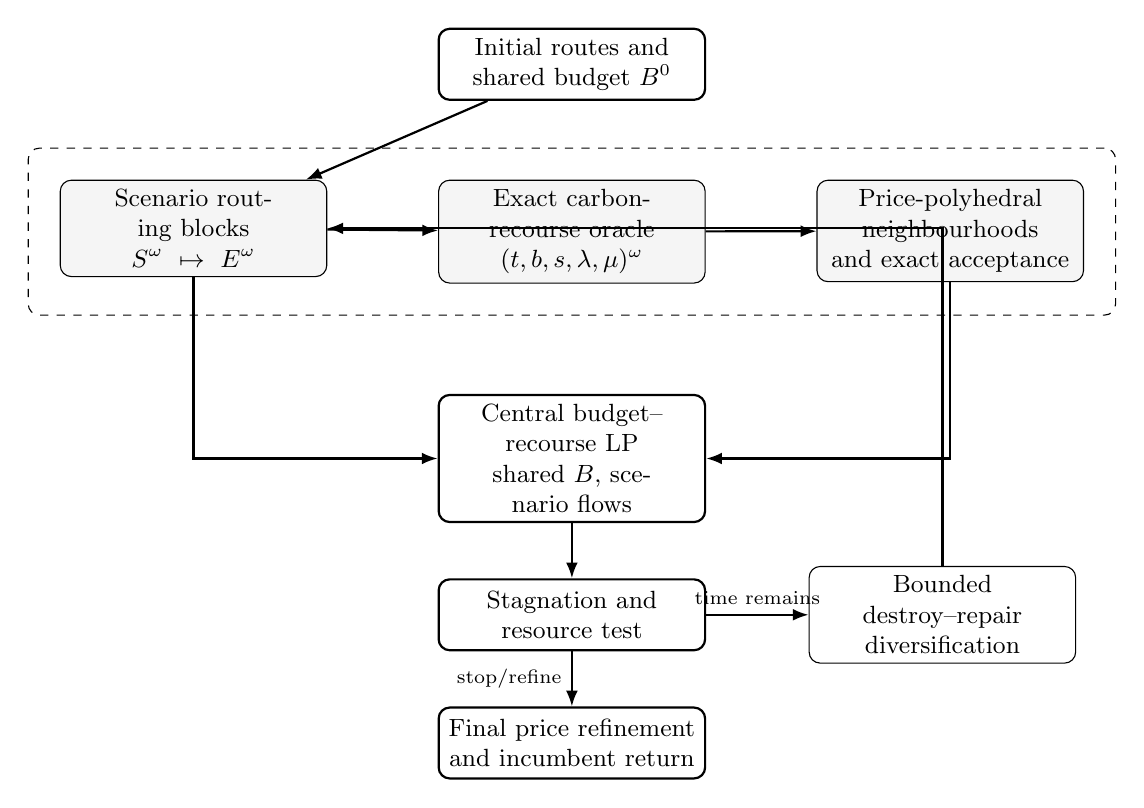
\begin{tikzpicture}[
 node distance=7mm and 9mm,
 box/.style={draw,rounded corners,align=center,text width=3.15cm,minimum height=9mm,font=\small},
 scen/.style={box,fill=gray!8},
 shared/.style={box,thick},
 arrow/.style={-{Latex[length=2mm]},thick}
]
\node[shared] (init) {Initial routes and shared budget $B^0$};
\node[scen,below left=10mm and 14mm of init] (route) {Scenario routing blocks\\$S^\omega\mapsto E^\omega$};
\node[scen,below=10mm of init] (oracle) {Exact carbon-recourse oracle\\$(t,b,s,\lambda,\mu)^\omega$};
\node[scen,below right=10mm and 14mm of init] (neigh) {Price-polyhedral neighbourhoods\\and exact acceptance};
\node[shared,below=14mm of oracle] (budget) {Central budget--recourse LP\\shared $B$, scenario flows};
\node[shared,below=of budget] (test) {Stagnation and resource test};
\node[box,right=13mm of test] (div) {Bounded destroy--repair\\diversification};
\node[shared,below=of test] (stop) {Final price refinement and incumbent return};
\draw[arrow] (init) -- (route);
\draw[arrow] (route) -- (oracle);
\draw[arrow] (oracle) -- (neigh);
\draw[arrow] (neigh) |- (budget);
\draw[arrow] (route) |- (budget);
\draw[arrow] (budget) -- (test);
\draw[arrow] (test) -- node[above,font=\scriptsize]{time remains} (div);
\draw[arrow] (div.north) |- (route.east);
\draw[arrow] (test) -- node[left,font=\scriptsize]{stop/refine} (stop);
\begin{scope}[on background layer]
\node[draw,dashed,rounded corners,fit=(route)(oracle)(neigh),inner sep=4mm] {};
\end{scope}
\end{tikzpicture}
\caption{PPBRC combines a monotone price-polyhedral coordination core with bounded post-stagnation diversification and final exact-objective refinement.}
\label{fig:ppbrc_flow}
\end{figure}

\subsection{Descent properties and convergence boundary}
\label{subsec:ppbrc_properties}

\begin{proposition}[Monotone objective sequence]
\label{prop:ppbrc_descent}
Suppose the routing block accepts only moves that strictly decrease \eqref{eq:ppbrc_true_scenario}, and the budget block solves \eqref{eq:budget_block_obj}--\eqref{eq:budget_block_domain} exactly without a penalised proximal term. Then the sequence of complete expected objective values generated by PPBRC is non-increasing.
\end{proposition}
\begin{proof}
At fixed $B^r$, every accepted scenario move decreases its weighted contribution to the complete objective, while all other scenarios remain unchanged. Hence the routing block gives $Z^{r+1/2}\le Z^r$. At fixed route emissions, $(B^r,t^r,b^r,s^r)$ is feasible for the budget block, whose exact optimum therefore satisfies $Z^{r+1}\le Z^{r+1/2}$. Combining the inequalities proves the claim.
\end{proof}

\begin{proposition}[Incumbent monotonicity under controlled diversification]
\label{prop:ppbrc_incumbent}
Suppose that non-improving working solutions may be accepted only inside the bounded diversification phase, while the stored incumbent is updated only after exact evaluation of the complete stochastic objective. Then the sequence of incumbent objective values generated by the complete PPBRC implementation is non-increasing.
\end{proposition}
\begin{proof}
The diversification trajectory may move to a worse working solution, but such a solution does not replace the incumbent. Every incumbent replacement is conditioned on a strict decrease under the complete objective, including exact carbon recourse and the feasible shared budget. Hence the best-so-far value cannot increase.
\end{proof}

\begin{corollary}[Objective-value convergence]
\label{cor:ppbrc_value_convergence}
If the complete objective has a finite lower bound, the objective sequence converges.
\end{corollary}
\begin{proof}
The sequence is non-increasing by Proposition~\ref{prop:ppbrc_descent} and bounded below, hence convergent.
\end{proof}

\begin{proposition}[Blockwise local optimality]
\label{prop:ppbrc_block_local}
Assume that the route neighbourhood is finite, the routing block terminates only after no strictly improving move remains in that neighbourhood for any scenario, the budget block is solved exactly, and deterministic tie-breaking excludes zero-improvement cycles. If PPBRC terminates without invoking a non-improving perturbation, its final solution is locally optimal with respect to the specified routing neighbourhood at the final budget and globally optimal in the budget--recourse block at the final route emissions.
\end{proposition}
\begin{proof}
The routing termination test excludes every strictly improving move in the enumerated neighbourhood at fixed budget. Exact solution of the budget block excludes every feasible budget and accounting-recourse change at fixed emissions. These two statements are precisely blockwise local optimality. They do not exclude an improving joint change that is not representable by one block at a time.
\end{proof}

These results concern descent and blockwise local optimality only. They do not imply convergence of the solution sequence, convexity of the full integer value function, or global optimality. The dual vector $\lambda^\omega$ is an exact subgradient of the recourse function at the current route emissions, not a global subgradient of the routing-optimised scenario value.

\subsection{Implementation and computational complexity}
\label{subsec:ppbrc_complexity}

For one scenario, the recourse network contains $|\mathcal D|$ balance nodes, $|\mathcal A^T|$ internal arcs, and $2|\mathcal D|$ external-market arcs. It is solved as a small capacitated minimum-cost flow. The budget block contains $|\mathcal D|$ shared budget variables and, per scenario, $|\mathcal A^T|+2|\mathcal D|$ accounting variables with $|\mathcal D|$ balance equations. Its size is therefore linear in $|\mathcal W|(|\mathcal A^T|+|\mathcal D|)$.

Depot--customer and customer--customer distances are precomputed, and route cost, payload, and load-dependent emission values are cached by scenario and route sequence.  Only the affected routes are recomputed after a candidate edit.  For relocate, swap, and 2-opt candidates, route-prefix demand summaries support incremental evaluation; best-position insertion limits the number of complete candidate plans. Compound cross-depot moves have a larger worst-case neighbourhood, so they are restricted to a short list of depot and route pairs selected by price gaps, congestion, and proximity. The expensive component is the combinatorial route search rather than either accounting LP. Scenario routing blocks are independent at fixed $B$ and are therefore parallelisable, with synchronisation required only before the central budget block.  The computational experiments distinguish this structural parallelism from realised speedup, which depends on the programming environment and scenario size.

%%=====================================================================
\section{Computational Experiments}
\label{sec:computational_experiments}

The experiments address five questions in turn: whether the model, its dual prices, and the algorithm are numerically consistent (Section~\ref{subsec:e1_verification}); whether price-polyhedral information improves search relative to external baselines (Section~\ref{subsec:e2_algorithm}); whether stochastic budget allocation has material value (Section~\ref{subsec:e3_stochastic_value}); how the operational and accounting recourse channels interact across a factorial design (Section~\ref{subsec:e4_recourse_interaction}); and whether the results carry over to public benchmark instances (Section~\ref{subsec:e5_public_benchmark}).  The algorithm architecture, external baselines, instance classes, scenario streams, and search seeds are all fixed before the reported runs.

\subsection{Experimental setup}
\label{subsec:experimental_setup}

Two datasets are used, each playing a role standard in this literature: a numerical-experiment dataset for controlled comparison, and a case-study dataset for external validity.  The numerical-experiment dataset comprises 94 reported instances (30 verification, 24 comparison, 8 stochastic-value, 32 sensitivity; Table~\ref{tab:frozen_data_suites}), together with 8 further instances used only for parameter calibration, all produced by a single instance-generation procedure that follows the classical multi-depot geometry of \citet{cordeau1997vrp}, the controlled clustered-instance methodology of \citet{uchoa2017benchmark}, the correlated-demand-shock decomposition surveyed by \citet{gendreau1996stochastic}, and the load-dependent fuel-consumption model of \citet{bektas2011pollution}.  Depot placement, core/boundary customer sampling, demand-shock generation, reference-emission construction, and transfer-network assembly are identical across every suite; the suites differ only in the scale and factor settings supplied to this procedure -- customer and depot counts, scenario-bank sizes, and, for E2 and E4, the carbon-network stratum or factorial cell -- as detailed in Table~\ref{tab:frozen_data_suites} and Appendix~\ref{app:scenario_generation}.

These differences follow directly from what each suite is designed to isolate, not from ad hoc regeneration.  The verification suite is kept small enough for exact solution by a mixed-integer solver; the comparison suite spans a size range wide enough to separate heuristic performance; the sensitivity suite fixes instance size entirely so that its $2^4$ factorial design attributes performance differences to the four manipulated factors rather than to incidental geometry changes.  Its 32 instances are the 16 factorial cells replicated twice, a count determined by the design rather than chosen for convenience.  All instance and scenario parameters are fixed in advance of algorithm comparison and are not revised after performance is observed.  Algorithm parameters -- neighbourhood limits, stopping rules, and wall-clock budgets -- are calibrated on the 8 separate instances mentioned above, which are generated by the same procedure but are disjoint from every instance on which results are reported; no parameter is tuned on an instance whose performance is subsequently reported.

The case-study dataset is the public Cordeau multi-depot benchmark itself \citep{cordeau1997vrp} (33 instances, used without modification), which Section~\ref{subsec:e5_public_benchmark} uses to test the routing engine against a recognised external benchmark (E5a) and to run the complete carbon-budget mechanism on a real, rather than self-generated, spatial and capacity structure (E5b); that section states precisely what each of these two roles does and does not establish.

Depot locations are placed on a mildly perturbed regular polygon.  Core customers are sampled around one home depot, whereas a pre-specified fraction of boundary customers is sampled around the midpoint of adjacent depots and is eligible for both.  Let $\bar q_i$ denote the base demand of customer $i$.  Scenario demands follow
\begin{equation}
 q_i^\omega
 =\bar q_i
 \exp\!\left(\sigma Z_{h(i)}^\omega-\frac{\sigma^2}{2}\right)
 \exp\!\left(\sigma_\varepsilon\varepsilon_i^\omega-
                  \frac{\sigma_\varepsilon^2}{2}\right),
 \label{eq:scenario_generator}
\end{equation}
where $Z^\omega$ is a depot-level Gaussian factor with equicorrelation $\rho$, and $\varepsilon_i^\omega$ is an independent customer shock.  The lognormal correction preserves the base demand in expectation.  Extreme draws are truncated or resampled only to maintain positivity and individual-vehicle feasibility.  Negative cross-depot correlation is permitted whenever the equicorrelation matrix is positive semidefinite.

The corporate budget is parameterised as
\begin{equation}
 B^{\mathrm{corp}}=\gamma_B E^0,
 \label{eq:budget_stringency}
\end{equation}
where $E^0$ is obtained from a deterministic home-depot angle-sweep construction under base demand.  The reference allocation is proportional to depot reference emissions, with lower and upper responsibility bounds equal to $45\%$ and $160\%$ of that allocation.  The internal transfer graph is a bidirectional ring; the five-depot classes include two additional bidirectional chords.  Arc frictions are directionally asymmetric, and capacities are scaled relative to the reference emissions of their incident depots.

Table~\ref{tab:parameter_values} lists the value of every parameter of the instance generator and of the carbon-account layer.  Values are held at these settings throughout, except for the factors that a given experiment deliberately varies: the budget factor $\gamma_B$ and transfer-capacity scale $\tau$ define the three carbon-network strata of the comparison suite, and the four factors of the sensitivity suite take the two levels listed in the final block.

\begin{table}[!htbp]
\centering
\caption{Parameter values used to generate the numerical-experiment dataset.}
\label{tab:parameter_values}
\footnotesize
\renewcommand{\arraystretch}{1.12}
\begin{tabular}{@{}lll@{}}
\toprule
Symbol & Meaning & Value \\
\midrule
\multicolumn{3}{@{}l}{\textit{Geometry and fleet}}\\
-- & Service region & $10\times10$ Euclidean square \\
-- & Depot layout & regular polygon, radius $0.35$ of region side \\
-- & Depot radial / angular perturbation & $\pm5\%$ of region side / $\pm30\%$ of half the inter-depot angle \\
-- & Customer cluster dispersion & $0.12$ of the mean inter-depot spacing \\
$\beta$ & Boundary-customer share & $0.20$ \\
$Q_k$ & Vehicle capacity (homogeneous fleet) & $100$ \\
$H_k$ & Maximum route duration & $6(2d^{\max}_d+1)$, with $d^{\max}_d$ the farthest member distance \\
-- & Target mean fleet utilisation (sizes $|\mathcal K_d|$) & $0.62$ \\
\midrule
\multicolumn{3}{@{}l}{\textit{Demand}}\\
$\bar q_i$ & Mean base demand & $12$ \\
-- & Within-depot base-demand c.v. & $0.30$ \\
-- & Between-depot demand-scale c.v. & $0.25$ \\
$\sigma$ & Depot-level shock c.v. in \eqref{eq:scenario_generator} & $0.25$ \\
$\sigma_\varepsilon$ & Customer-level shock c.v. in \eqref{eq:scenario_generator} & $0.10$ \\
$\rho$ & Cross-depot equicorrelation & $0.25$ \\
-- & Distribution-shift bank: depot shock & standardised Student-$t_5$ \\
-- & Distribution-shift bank: surge regime & probability $0.05$, multiplier $1.5$ \\
\midrule
\multicolumn{3}{@{}l}{\textit{Emissions, budget, and carbon market}}\\
$\theta$ & Fuel-to-emission conversion & $1.0$ \\
$\rho_k^0,\rho_k^Q$ & Empty- and full-load fuel rates & $0.9$, $1.5$ \\
$\gamma_B$ & Corporate budget factor in \eqref{eq:budget_stringency} & $1.00$ (baseline) \\
$\underline B_d,\overline B_d$ & Depot responsibility bounds & $0.45$, $1.60$ times the reference allocation \\
$p^{\mathrm{buy}},p^{\mathrm{sell}}$ & External purchase and sale prices & $9$, $2$ \\
\midrule
\multicolumn{3}{@{}l}{\textit{Internal transfer network}}\\
$\mathcal A^T$ & Topology & bidirectional ring ($+2$ chords when $|\mathcal D|=5$) \\
$\kappa_{dd'}$ & Arc friction & $(0.15+0.35\,\tilde d_{dd'})(1\pm0.15)$, $\tilde d$ normalised depot distance \\
$\overline T_{dd'}$ & Arc capacity & $\tau\cdot\tfrac12(E^0_d+E^0_{d'})$ \\
$\tau$ & Transfer-capacity scale & $1.00$ (baseline) \\
\midrule
\multicolumn{3}{@{}l}{\textit{Factors varied by design}}\\
$(\gamma_B,\tau)$ & Comparison-suite carbon-network strata & $(0.90,0.60)$, $(1.00,1.00)$, $(1.10,1.40)$ \\
$\sigma$ & Sensitivity factor: demand c.v. & $0.15$ or $0.35$ \\
$\rho$ & Sensitivity factor: cross-depot correlation & $-0.25$ or $0.55$ \\
$\beta$ & Sensitivity factor: boundary share & $0.10$ or $0.30$ \\
$\tau$ & Sensitivity factor: transfer-capacity scale & $0.60$ or $1.40$ \\
\midrule
\multicolumn{3}{@{}l}{\textit{Random streams}}\\
-- & Stream bases (geometry / train / validation / test / shift) & $10^6$, $2\times10^6$, $3\times10^6$, $4\times10^6$, $5\times10^6$ \\
-- & Search seeds & $\{91001,\dots,91005\}$ \\
\bottomrule
\end{tabular}
\end{table}

Table~\ref{tab:frozen_data_suites} summarises the resulting suites.  For E3, the 20-, 50-, and 100-scenario training samples are nested prefixes of the same 100-scenario bank.  The validation bank is used only to select the training sample size and stopping settings.  The final test bank is sealed until the algorithm, baselines, and parameters have been fixed.  A separate heavy-tailed regime-switching bank is used only for supplementary distribution-shift analysis and does not replace the main same-distribution test bank.

\begin{table}[!htbp]
\centering
\caption{Instance and scenario suites used in the reported experiments. A further 8 calibration instances, generated by the same procedure at $|\mathcal C|\in\{20,50,75,100\}$ and $|\mathcal D|\in\{3,5\}$, are used only to set algorithm parameters and are reported nowhere.}
\label{tab:frozen_data_suites}
\footnotesize
\renewcommand{\arraystretch}{1.12}
\begin{tabular}{@{}llllll@{}}
\toprule
Suite & Instances & $|\mathcal C|$ & $|\mathcal D|$ & Training scenarios & Independent evaluation scenarios \\
\midrule
Verification (Section~\ref{subsec:e1_verification})    & 30 & 10, 20, 30 & 2, 3 & 2--10 & -- \\
Comparison (Section~\ref{subsec:e2_algorithm})         & 24 & 20, 50, 75, 100 & 3, 5 & 20 & -- \\
Stochastic value (Section~\ref{subsec:e3_stochastic_value}) & 8 & 20, 50, 75, 100 & 3, 5 & 20/50/100 & 200 validation $+$ 800 test $+$ 200 shift \\
Sensitivity (Section~\ref{subsec:e4_recourse_interaction})  & 32 & 60 & 3 & 50 & 100 validation $+$ 400 test \\
Public benchmark (Section~\ref{subsec:e5_public_benchmark}) & 33/11 & 50--360 & 2--9 & 1/50 & 200 validation $+$ 800 test \\
\bottomrule
\end{tabular}
\end{table}

The comparison suite contains three pre-specified carbon-network strata for every size class: a tight-budget/low-capacity stratum, a balanced stratum, and a loose-budget/high-capacity stratum.  The sensitivity suite uses a replicated $2^4$ design over demand coefficient of variation ($0.15$ or $0.35$), cross-depot correlation ($-0.25$ or $0.55$), boundary-customer share ($0.10$ or $0.30$), and transfer-capacity scale ($0.60$ or $1.40$).  Every generated instance is retained; mechanism diagnostics describe the resulting strata but are never used to remove an unfavourable instance.  The public-benchmark experiment provides external validity using the Cordeau MDVRP instances: all 33 are used for an unmodified deterministic routing regression, while 11 pre-specified instances spanning 50--360 customers and 2--9 depots additionally receive the stochastic-demand and carbon-account overlay.  The original public coordinates, depots, mean demands, capacities, route-duration limits, and vehicle limits are never perturbed or filtered.

Before evaluating solution quality, each instance class is described by deficit--surplus coexistence, depot-price dispersion, transfer use, saturated arcs, and the incidence of external purchase and sale.  These diagnostics establish which mechanisms are active in a pre-specified class; they are not an ex-post selection rule.

\begin{table}[!htbp]
\centering
\caption{Mechanism-activation diagnostics by pre-specified instance class.}
\label{tab:mechanism_activation}
\resizebox{\textwidth}{!}{%
\begin{tabular}{lrrrrrr}
\toprule
Class & Deficit--surplus coexistence (\%) & Mean price dispersion & Transfer-use scenarios (\%) & Saturated arcs (\%) & Purchase scenarios (\%) & Sale scenarios (\%)\\
\midrule
\multicolumn{7}{c}{\textit{To be filled from the frozen instances without ex-post filtering}}\\
\bottomrule
\end{tabular}}
\end{table}

All heuristic comparisons use identical hardware, total wall-clock limits, training scenarios, deterministic reference starts, and the five frozen search seeds $\{91001,91002,91003,91004,91005\}$.  External baselines receive the same exact load-dependent route evaluator, carbon-recourse oracle, and shared-budget feasibility recovery as PPBRC.  SAA-ALNS uses a conventional reactive destroy--repair search without price-polyhedral guidance.  PH-ALNS uses scenario budget copies and multiplier-based consensus coordination; because it is a heuristic adaptation for an integer routing problem, both its feasible recovered objective and its budget-consensus residual are reported.  PPBRC-core and complete PPBRC use the same total time limit, with the latter allocating only the unused post-stagnation budget to controlled diversification.  We report best, mean, median, standard deviation, wall-clock time, paired differences, and anytime performance.  Paired Wilcoxon tests are descriptive; raw paired differences and effect sizes remain primary.  Every reported solution is evaluated with the complete objective \eqref{eq:ppbrc_true_scenario} and exact accounting recourse.

\subsection{Verification against exact solutions}
\label{subsec:e1_verification}

Small deterministic equivalents use $|\mathcal C|\in\{10,20,30\}$, $|\mathcal D|\in\{2,3\}$, and $|\mathcal W|\in\{2,4,6,8,10\}$, giving 30 instances in total. A MILP solver provides a proven optimum or the best valid bound within the stated time limit; cells in which no integer-feasible incumbent is found within that limit are reported as such rather than silently omitted, and the heuristic is then assessed only against the valid bound. Before these main runs, tiny multi-vehicle instances are cross-checked with two independent exact formulations: the direct arc--payload deterministic-equivalent MILP in Section~\ref{subsec:mathematical_formulation}, and an exact route-plan extensive form obtained by enumerating every feasible customer assignment, vehicle partition, and route sequence in each scenario.  Agreement between these formulations isolates modelling and indexing errors that would not be detected by re-evaluating a heuristic solution with the same route code.

The verification script independently checks customer coverage, route continuity, the number of active vehicles, capacity, route duration, payload conservation, depot emissions, account balance, transfer capacity, first-stage non-anticipativity, and the absence of simultaneous buying and selling above tolerance. For every recourse call it also checks primal--dual equality, price bounds, and complementary conditions on unused, interior, and saturated transfer arcs.

\begin{table}[!htbp]
\centering
\caption{Exact and numerical verification on small CBAR-MDVRP instances. All entries are populated from solver output.}
\label{tab:e1_verification}
\resizebox{\textwidth}{!}{%
\begin{tabular}{rrrllrrrrrr}
\toprule
$|\mathcal C|$ & $|\mathcal D|$ & $|\mathcal W|$ & MILP status & PPBRC status & Gap (\%) & Exact-form error & Max balance error & Primal--dual error & Feasibility (\%) & Time (s)\\
\midrule
\multicolumn{11}{c}{\textit{To be filled from verified computational output}}\\
\bottomrule
\end{tabular}}
\end{table}

Primary metrics are mean and worst optimality gap, the maximum difference between the two independent exact formulations, maximum component-wise objective error, maximum recourse primal--dual error, feasibility rate, and wall-clock time. The implementation target is an exact-form discrepancy, account-balance residual, and recourse primal--dual residual below $10^{-6}$; any run exceeding the declared tolerance is classified as an implementation failure rather than a feasible observation.  E1 also reports the number of active vehicles so that a nominal multi-depot test cannot silently collapse to one route per depot. No zero-gap or exact-recovery claim is made before the results are available.

\subsection{Comparative algorithm performance}
\label{subsec:e2_algorithm}


The comparison suite contains 24 instances: $|\mathcal C|\in\{20,50,75,100\}$, $|\mathcal D|\in\{3,5\}$, and three pre-specified carbon-network strata per size class.  Every stochastic instance contains 20 training scenarios.  Each stochastic method is run with the five pre-specified search seeds under identical anytime checkpoints and a common final wall-clock limit.  The primary external comparison is complete PPBRC versus SAA-ALNS and PH-ALNS; PPBRC-core, Cost-only coordination, and Price-guided routing only are retained as internal mechanism controls.

This experiment separates external competitiveness from internal mechanism attribution. All methods use the same complete objective and exact carbon-recourse evaluation:
\begin{enumerate}
\item \textbf{SAA-ALNS}: a reactive destroy--repair search with random, worst, and related removals, greedy and regret-2 repair, simulated-annealing acceptance, and periodic exact optimisation of the shared budget.
\item \textbf{PH-ALNS}: a heuristic progressive-hedging adaptation with scenario-specific budget copies, exact recourse subgradients in projected proximal updates, adaptive penalty balancing, scenario ALNS, and exact feasible nonanticipative recovery.
\item \textbf{Cost-only coordination}: the PPBRC block architecture without depot prices or congestion multipliers.
\item \textbf{Price-guided routing only}: the price-polyhedral routing block with the initial budget fixed.
\item \textbf{PPBRC-core}: the monotone single-trajectory price-polyhedral routing and exact budget-coordination engine.
\item \textbf{PPBRC}: PPBRC-core with bounded post-stagnation destroy--repair diversification followed by final price-polyhedral refinement.
\end{enumerate}
Sequential, equal-allocation, and uniform-price policies remain simple managerial benchmarks; compound cross-depot neighbourhoods and restart portfolios are retained only in the appendix because earlier equal-time pilots did not show stable gains.

\begin{table}[!htbp]
\centering
\caption{External-baseline pilot over four independent instances and two search seeds per instance. Objectives are feasible values under one shared budget; PH residual is the mean disagreement of scenario budget copies before feasible recovery. These development results are not the final publication experiment.}
\label{tab:e2_external_pilot}
\resizebox{\textwidth}{!}{%
\begin{tabular}{rllrrrr}
\toprule
Limit (s) & Method & Mean objective & Std. & Mean case-best gap (\%) & Mean runtime (s) & PH residual\\
\midrule
1.5 & PH-ALNS & \textbf{102.886} & 10.582 & \textbf{3.849} & 1.517 & 0.261\\
1.5 & PPBRC-core & 105.642 & 14.299 & 6.493 & 1.502 & 0\\
1.5 & SAA-ALNS & 111.369 & 15.100 & 12.147 & 1.522 & 0\\
\midrule
4.0 & PPBRC-core & \textbf{92.951} & 7.201 & \textbf{0.088} & 2.075 & 0\\
4.0 & PH-ALNS & 97.838 & 10.272 & 5.204 & 4.018 & 0.331\\
4.0 & SAA-ALNS & 98.440 & 9.877 & 5.898 & 4.023 & 0\\
\bottomrule
\end{tabular}}
\end{table}

At 1.5 seconds, PH-ALNS has the lowest mean recovered objective, but its scenario budget copies remain materially non-consensual; only the exactly recovered shared-budget solution is treated as feasible. PPBRC-core beats SAA-ALNS in six of eight paired runs, although the pilot sample is too small for a conclusive test. At four seconds, PPBRC-core beats SAA-ALNS in all eight runs, with a mean reduction of 5.35\% ($p=0.007812$), and beats PH-ALNS in seven of eight runs, with a mean reduction of 4.74\% ($p=0.015625$). The core terminates after approximately 2.1 seconds on average, whereas the external baselines consume almost the full four-second allowance.

A longer eight-second diagnostic nevertheless shows that SAA-ALNS can eventually overtake the monotone core on three of four instances because the latter stops at a blockwise local optimum and leaves the remaining time unused. This motivates the controlled diversification phase in the complete implementation.

\begin{table}[!htbp]
\centering
\caption{Controlled-diversification pilot at a four-second total limit over four instances and two search seeds.}
\label{tab:e2_diversification_pilot}
\begin{tabular}{lrrrr}
\toprule
Method & Mean objective & Std. & Mean case-best gap (\%) & Mean runtime (s)\\
\midrule
PPBRC & \textbf{90.811} & 7.421 & \textbf{0.260} & 3.975\\
PPBRC-core & 92.951 & 7.201 & 2.681 & 2.024\\
SAA-ALNS & 97.850 & 9.375 & 8.036 & 4.024\\
\bottomrule
\end{tabular}
\end{table}

Complete PPBRC improves on SAA-ALNS by 6.98\% on average, with seven wins and one loss ($p=0.015625$). Relative to PPBRC-core, the controlled phase reduces the mean objective by 2.29\%, with six wins, one tie, and one loss ($p=0.078125$). An eight-second, one-seed diagnostic gives mean objectives of 88.517 for PPBRC, 90.830 for SAA-ALNS, and 92.951 for PPBRC-core; PPBRC wins three of four cases against SAA-ALNS. These results justify controlled diversification as a practical post-stagnation mechanism, but the final paper will rely on a larger frozen instance set, multiple seeds, and longer time limits.

The external-baseline comparison changes the interpretation of the algorithmic contribution. Generic ALNS supplies strong early and long-horizon diversification; the price-polyhedral core supplies efficient marginal screening and exact budget feedback. The complete method combines these roles without treating destroy--repair mechanics as the theoretical novelty. The final experiment reports anytime curves, oracle calls, budget updates, PH consensus residuals, and paired solution-quality statistics in addition to final objective values.

\subsection{Value of the stochastic carbon-budget allocation}
\label{subsec:e3_stochastic_value}


This experiment uses eight geometries with $|\mathcal C|\in\{20,50,75,100\}$ and $|\mathcal D|\in\{3,5\}$.  For each geometry, the stochastic solution is estimated from nested training samples of 20, 50, and 100 scenarios.  Training-sample selection is based on 200 independent validation scenarios.  The selected policy is then evaluated once on 800 sealed same-distribution scenarios.  A separate 200-scenario heavy-tailed regime-switching bank assesses distribution-shift sensitivity in the appendix.  VSS and EVPI are reported in sample, whereas implementable policy comparisons are based on the independent validation and test banks.

We compare six first-stage policies: equal allocation, expected-demand allocation,
reference-emission allocation, the expected-value deterministic solution, the
stochastic CBAR solution, and a wait-and-see solution that may choose $B$ after
observing each scenario. Let $Z_{\mathrm{EV}}$ be the expected cost obtained by
implementing the expected-value budget and reoptimising second-stage decisions,
$Z_{\mathrm{SP}}$ the stochastic-programme value, and $Z_{\mathrm{WS}}$ the
wait-and-see value. For this minimisation problem,
\begin{equation}
 \mathrm{VSS}=Z_{\mathrm{EV}}-Z_{\mathrm{SP}}\ge0,
 \qquad
 \mathrm{EVPI}=Z_{\mathrm{SP}}-Z_{\mathrm{WS}}\ge0.
 \label{eq:vss_evpi}
\end{equation}

A first four-case implementation pilot used four training scenarios and six
independent test scenarios per case. Table~\ref{tab:e3_stochastic} reports the
cross-case means. The stochastic solution has a large in-sample advantage but
does not dominate simple reference policies out of sample. This discrepancy is
treated as evidence of small-sample overfitting rather than as a favourable
result to be hidden.

\begin{table}[!htbp]
\centering
\caption{Stochastic budget allocation and independent test performance (pilot).}
\label{tab:e3_stochastic}
\resizebox{\textwidth}{!}{%
\begin{tabular}{lrrrrrrrr}
\toprule
Policy & Train cost & Test cost & Test Std. & Buy cost & Sale revenue & Transfer & Bound hits & Price dispersion\\
\midrule
Equal allocation & 104.822 & 105.574 & 30.075 & 30.956 & 3.836 & 2.786 & 0.50 & 1.710\\
Expected-demand allocation & 103.934 & 107.239 & 30.635 & 32.638 & 4.243 & 3.168 & 0.25 & 1.951\\
Reference-emission allocation & 101.178 & 110.138 & 33.132 & 35.512 & 4.725 & 3.194 & 0.00 & 1.610\\
Expected-value solution & 106.119 & 118.937 & 33.790 & 46.005 & 7.113 & 3.575 & 0.25 & 2.365\\
Stochastic CBAR solution & \textbf{83.546} & 111.205 & 33.152 & 37.170 & 5.073 & 3.083 & 0.25 & 1.813\\
Wait-and-see & 75.222 & \textbf{89.904} & \textbf{21.905} & \textbf{17.753} & 3.983 & \textbf{0.996} & 0.96 & \textbf{0.620}\\
\bottomrule
\end{tabular}}
\end{table}

On the training samples, all four cases satisfy the expected ordering
$Z_{\mathrm{WS}}\le Z_{\mathrm{SP}}\le Z_{\mathrm{EV}}$. The mean values are
\[
 \mathrm{VSS}=22.573\;(27.31\%\text{ of }Z_{\mathrm{SP}}),
 \qquad
 \mathrm{EVPI}=8.324\;(10.01\%\text{ of }Z_{\mathrm{SP}}).
\]
These sample-based quantities demonstrate that the first-stage decision can be
active, but they overstate the implementable value when the scenario sample is
small. In the independent test set, the stochastic policy is 5.33\% more costly
than equal allocation and 0.97\% more costly than reference-emission allocation
in this pilot.

We therefore conducted a separate scenario-sample-size diagnostic on three
independent geometries. The test set was held fixed while the training sample
increased from four to twelve scenarios. Table~\ref{tab:e3_sample_size} shows
that the stochastic policy gradually overtakes the reference-emission policy,
but the test improvement remains modest.

\begin{table}[!htbp]
\centering
\caption{Effect of the number of training scenarios on independent test cost (pilot).}
\label{tab:e3_sample_size}
\begin{tabular}{crrrr}
\toprule
Training scenarios & Policy & Mean test cost & Improvement vs. reference (\%) & External buy cost\\
\midrule
\multirow{3}{*}{4}
 & Reference-emission & 114.059 & 0.000 & 33.627\\
 & Expected-value & 118.286 & -3.459 & 38.298\\
 & Stochastic CBAR & 114.198 & 0.036 & 34.188\\
\midrule
\multirow{3}{*}{8}
 & Reference-emission & 106.535 & 0.000 & 26.356\\
 & Expected-value & 108.131 & -1.337 & 27.990\\
 & Stochastic CBAR & 106.395 & 0.183 & 26.272\\
\midrule
\multirow{3}{*}{12}
 & Reference-emission & 103.170 & 0.000 & 23.207\\
 & Expected-value & 105.063 & -1.700 & 25.011\\
 & Stochastic CBAR & \textbf{102.933} & \textbf{0.319} & \textbf{23.126}\\
\bottomrule
\end{tabular}
\end{table}

The pilot therefore supports two more cautious conclusions. First, optimising
against demand uncertainty can improve depot-budget allocation, but its
out-of-sample value is materially smaller than the in-sample VSS. Second, the
final experiment must use a substantially larger training sample, report an
independent test set, and include a scenario-sample-size stability check.
Budget vectors and expected depot prices will be reported alongside VSS and
EVPI. The wait-and-see policy remains an information benchmark rather than an
implementable policy.

\subsection{Sensitivity analysis of operational and accounting recourse}
\label{subsec:e4_recourse_interaction}

A $2\times2$ design switches operational recourse and internal-accounting
recourse on or off. Operational recourse is disabled by fixing each customer
to its home depot; accounting recourse is disabled by setting all internal
transfer capacities to zero. External trading remains available in all cases
to preserve complete recourse. Let $Z_{ab}$ denote the expected cost, where
$a$ indicates operational recourse and $b$ indicates internal accounting
recourse. Define
\begin{equation}
 V_{\mathrm{op}}=Z_{00}-Z_{10},\qquad
 V_{\mathrm{acc}}=Z_{00}-Z_{01},\qquad
 V_{\mathrm{joint}}=Z_{00}-Z_{11},
 \label{eq:recourse_values}
\end{equation}
with interaction
\begin{equation}
 I=V_{\mathrm{joint}}-V_{\mathrm{op}}-V_{\mathrm{acc}}.
 \label{eq:interaction_index}
\end{equation}
Positive $I$ indicates complementarity relative to additivity, whereas negative
$I$ indicates substitution.

The six-case structural pilot varies demand variability, demand correlation,
boundary-customer availability, transfer friction, transfer capacity, and
budget stringency. The average regime outcomes are reported in
Table~\ref{tab:e4_interaction}.

\begin{table}[!htbp]
\centering
\caption{Operational--accounting recourse regimes (pilot).}
\label{tab:e4_interaction}
\begin{tabular}{ccrrrrr}
\toprule
Operational & Accounting & Mean cost & Cross-depot (\%) & Internal transfer & External buy & Price dispersion\\
\midrule
No & No & 84.603 & 0.000 & 0.000 & 1.394 & 2.483\\
Yes & No & 76.061 & 4.444 & 0.000 & 0.937 & 2.842\\
No & Yes & 77.712 & 0.000 & 0.227 & 0.645 & 2.122\\
Yes & Yes & \textbf{69.617} & 7.361 & 0.746 & \textbf{0.430} & \textbf{1.497}\\
\bottomrule
\end{tabular}
\end{table}

Across the six cases, operational recourse reduces expected cost by 8.541 on
average, accounting recourse by 6.891, and their joint use by 14.985. The
average interaction is close to zero,
\[
 I=-0.447\quad(-0.22\%\text{ of }Z_{00}),
\]
but the case-level signs are heterogeneous: three cases show complementarity
and three show substitution. Hence neither mechanism universally dominates or
universally complements the other. In the pilot, cases with more boundary
customers and higher demand variability are more often associated with
positive interaction, whereas highly restrictive or readily substitutable
settings can produce negative interaction. Because the factors are confounded
in this small fractional design, these associations are treated as hypotheses
for the frozen factorial experiment, not as causal conclusions.

The joint regime also lowers mean external purchases from 1.394 to 0.430 and
reduces price dispersion from 2.483 to 1.497. These outcomes are consistent
with the interpretation that physical reassignment and allowance transfer
jointly absorb depot-level carbon imbalances. All sensitivity runs are monotone; the
maximum account residual is $1.78\times10^{-15}$ and the maximum recourse
primal--dual discrepancy is $1.51\times10^{-14}$.

When the fully pooled regime is included as an institutional benchmark, its
recourse cost is computed from \eqref{eq:pooled_recourse} rather than from a
zero-cost complete transfer network. The pooled benchmark therefore reports
aggregate external trading and the common price, but not an arbitrary
depot-to-depot transfer volume; see Remark~\ref{rem:canonical_pooling}.


\subsection{External validation on public benchmark instances}
\label{subsec:e5_public_benchmark}

The synthetic suites are necessary for controlled activation of demand risk,
carbon-budget stringency, and transfer-network congestion, but they do not by
themselves establish external routing credibility.  We therefore add a
separate public-benchmark layer based on the 33 Cordeau MDVRP instances
\citep{cordeau1997vrp}.  The public source files are used without changing
customer coordinates, depot coordinates, mean demands, vehicle capacities,
route-duration limits, or maximum vehicle counts.  The conversion script,
source hashes, converted-file hashes, scenario seeds, and solution-file parsing
status are archived with the computational supplement.

\paragraph{E5a: regression to the classical MDVRP.}
The first test removes every paper-specific extension: demand is deterministic,
the carbon and accounting terms are disabled, and the objective is the original
Euclidean route duration.  The routing engine is run on all 33 public instances
and compared with the published best-known solution (BKS).  This test validates
route representation, multi-depot assignment, vehicle counting, capacity,
route duration, and the diversification substrate.  It is not presented as
evidence for the stochastic carbon-budget mechanism.

\begin{table}[!htbp]
\centering
\caption{Routing regression on the public MDVRP benchmark (E5a), over all 33 Cordeau instances.}
\label{tab:e5a_public_routing}
\resizebox{\textwidth}{!}{%
\begin{tabular}{lrrrrrr}
\toprule
Instance class & Instances & Customers & Depots & Best gap to BKS (\%) & Mean gap (\%) & Feasible runs (\%)\\
\midrule
Small  &  & 50--80   & 2--5 & \multicolumn{3}{c}{\textit{To be filled from frozen runs}}\\
Medium &  & 100      & 2--4 & \multicolumn{3}{c}{\textit{To be filled from frozen runs}}\\
Large  &  & 160--360 & 4--9 & \multicolumn{3}{c}{\textit{To be filled from frozen runs}}\\
\bottomrule
\end{tabular}}
\end{table}

\paragraph{E5b: CBAR on public routing backbones.}
The complete CBAR-MDVRP is evaluated on the pre-specified subset
\{p01,p02,p03,p12,p04,p05,p06,p07,p15,p18,p21\}.  Because the public
instances are deterministic classical MDVRP instances, they carry none of
the attributes this paper's model requires: they have no demand
uncertainty, no emission accounting, no carbon budget, and no internal
transfer network.  These attributes are therefore added by the deterministic
conversion set out in Table~\ref{tab:public_augmentation}, which retains
every original attribute unchanged and only appends new ones.  The
conversion is a function of published data alone -- coordinates, mean
demands, capacities, and, where parseable, the published best-known route --
so it involves no tuning and can be reproduced exactly from the public files.

\begin{table}[!htbp]
\centering
\caption{Attributes retained from, and added to, the public Cordeau instances in E5b.}
\label{tab:public_augmentation}
\footnotesize
\renewcommand{\arraystretch}{1.12}
\begin{tabular}{@{}lp{0.62\textwidth}@{}}
\toprule
Attribute & Treatment \\
\midrule
\multicolumn{2}{@{}l}{\textit{Retained from the public instance, unchanged}}\\
Customer and depot coordinates & used as published; never perturbed, deleted, or re-selected \\
Mean customer demands & become the base demands $\bar q_i$ of \eqref{eq:scenario_generator} \\
Vehicle capacity, route-duration limit, vehicle count & used as published \\
Depot eligibility & unrestricted across all public depots, as in the classical MDVRP \\
\midrule
\multicolumn{2}{@{}l}{\textit{Added by the conversion}}\\
Demand uncertainty & \eqref{eq:scenario_generator} applied to the published means, with $\sigma=0.25$, $\sigma_\varepsilon=0.10$, $\rho=0.25$; a draw is resampled only if it exceeds vehicle capacity \\
Scenario banks & 50 optimisation, 200 validation, 800 sealed test scenarios, from disjoint random streams \\
Emissions & load-dependent model of \citet{bektas2011pollution} with $\theta=1$, $\rho_k^0=0.9$, $\rho_k^Q=1.5$ \\
Reference emission $E^0$ & emission of the published best-known route under mean demand; where the published solution file cannot be parsed, a fully specified nearest-depot angular-sweep construction is used instead and is flagged as such, never reported as a best-known route \\
Corporate budget & $B^{\mathrm{corp}}=\gamma_B E^0$ with $\gamma_B\in\{0.90,1.00,1.10\}$; depot bounds at $0.45$ and $1.60$ times the emission-proportional allocation, as in the generated instances \\
Transfer network & bidirected Euclidean minimum spanning tree over the public depot coordinates, augmented by each depot's nearest omitted neighbour \\
Transfer friction and capacity & $\kappa_{dd'}=0.15+0.35\,\tilde d_{dd'}$ in normalised depot distance; $\overline T_{dd'}=\tau\cdot\tfrac12(E^0_d+E^0_{d'})$ with $\tau\in\{0.60,1.00,1.40\}$ \\
External prices & $p^{\mathrm{buy}}=9$, $p^{\mathrm{sell}}=2$, as in the generated instances \\
\bottomrule
\end{tabular}
\end{table}

Two differences from the generated instances are deliberate.  The transfer
network is a minimum spanning tree rather than a ring, because the public
depot coordinates are irregular and a ring imposed on them would be an
arbitrary artefact; and depot eligibility is unrestricted rather than
governed by \eqref{eq:depot_flexibility}, because restricting it would alter
the public routing problem.  Every other component uses the same functional
form and the same parameter values as Table~\ref{tab:parameter_values}, so
differences in results between the two datasets cannot be attributed to a
change in the carbon model.  PPBRC, PPBRC-core, SAA-ALNS, and PH-ALNS are compared
under the same time and seed protocol used in the comparison experiment. The original MDVRP BKS is
not used to compute an optimality gap for this augmented objective because the
uncertainty, emissions, and accounting recourse change the problem.

\begin{table}[!htbp]
\centering
\caption{Algorithm comparison on public Cordeau instances with the carbon-account overlay (E5b).}
\label{tab:e5b_public_cbar}
\resizebox{\textwidth}{!}{%
\begin{tabular}{lrrrrrrrr}
\toprule
Method & Train objective & Test objective & Test SE & Relative test cost (\%) & External buy & Internal transfer & Cross-depot (\%) & Time (s)\\
\midrule
SAA-ALNS   & \multicolumn{8}{c}{\textit{To be filled from the sealed public-backbone experiment}}\\
PH-ALNS    & \multicolumn{8}{c}{\textit{To be filled from the sealed public-backbone experiment}}\\
PPBRC-core & \multicolumn{8}{c}{\textit{To be filled from the sealed public-backbone experiment}}\\
PPBRC      & \multicolumn{8}{c}{\textit{To be filled from the sealed public-backbone experiment}}\\
\bottomrule
\end{tabular}}
\end{table}

The two public tests answer different questions. E5a measures compatibility
with a recognised routing benchmark and can be compared with published BKS
values. E5b measures algorithmic and policy performance for the new CBAR
problem on externally supplied spatial and capacity structures. A favourable
E5a result cannot validate the carbon model, and an E5b objective cannot be
compared numerically with the original MDVRP BKS.

\subsection{Claims-to-evidence discipline}
\label{subsec:claims_evidence}

Each experiment supports a specific and bounded claim.  The verification experiment establishes numerical consistency and small-instance solution quality, but cannot establish scalability.  The comparison experiment identifies the contribution of price-polyhedral coordination on the tested instances, but cannot prove dominance on all instances.  The stochastic-value experiment quantifies the value of stochastic optimisation under the chosen scenario model, and does not establish robustness to misspecified distributions.  The sensitivity experiment identifies empirical complementarity or substitution between the two recourse channels, and does not prove a universal sign for $I$.  Within the public-benchmark experiment, E5a establishes routing compatibility with a recognised MDVRP benchmark but does not validate the carbon-account extension, and E5b provides external spatial and capacity structure for the augmented model but does not inherit the original MDVRP best-known solutions, because its objective and information structure differ.

%%=====================================================================
\section{Conclusion}
\label{sec:conclusion}

This study develops the CBAR-MDVRP, a two-stage stochastic routing model in
which headquarters delegates depot-level carbon budgets before demand is
observed and coordinates operational and accounting recourse after demand is
realised.  The formulation distinguishes physical recourse through
customer--depot reassignment and route reconstruction from accounting recourse
through a capacity-constrained internal carbon-credit network and residual
external trading.  This distinction makes the first-stage allocation
economically meaningful whenever depot responsibilities and demand risks are
heterogeneous and carbon transfers are not frictionless.

For fixed route emissions, the carbon-account component is a capacitated
minimum-cost transshipment problem.  Its dual defines an extended price
polyhedron whose depot prices measure marginal recourse costs and whose
capacity multipliers identify congested internal-transfer channels.  These
quantities provide exact local information for the continuous recourse
function, including price bounds, transfer complementarity conditions, and a
subgradient lower bound for route moves.  They do not make the complete
integer routing value function convex.

PPBRC uses this structure in two coordinated blocks.  At a fixed shared
budget, scenario routing searches are guided by depot prices and congestion
multipliers, while shortlisted moves are accepted only after exact recourse
re-evaluation.  At fixed scenario emissions, a central linear programme
optimises the non-anticipative budget and all accounting-recourse decisions.
The resulting monotone core converges in objective value and terminates at a
blockwise local optimum relative to the specified route neighbourhoods; it
does not provide a global-optimality guarantee.  Restricted compound
cross-depot moves are included to reduce the local-optimality limitations of
single-customer edits.

The computational design separates four questions: exact model and dual
verification, the incremental value of price-polyhedral guidance and compound
neighbourhoods, the value of stochastic budget allocation, and the interaction
between operational and accounting recourse.  Mechanism-activation diagnostics
are reported before performance comparisons so that weak or degenerate
parameter regimes remain visible rather than being removed after observing the
results.  The fully pooled benchmark is implemented through its aggregate
settlement representation to avoid economically meaningless zero-cost
circulation flows.

The framework remains limited to a single planning period, a finite demand
scenario set, centralised decision making, and exogenous external carbon
prices.  Multi-period banking and borrowing, endogenous internal incentives,
distributionally robust demand models, and decentralised depot behaviour are
natural extensions, but each would alter the coordination problem rather than
serve as a minor add-on to the present model.
%%=====================================================================
\appendix

\section{PPBRC implementation details}
\label{app:ppbrc_details}

\subsection{Initial routes and initial budget}
Home-depot routes are built by regret insertion under capacity and route-duration constraints, followed by deterministic relocate, swap, and 2-opt improvement. The reference-emission budget is
\[
 B_d^0=B^{\mathrm{corp}}\frac{\sum_\omega\pi_\omega E_d^{0,\omega}}{\sum_{h\in\mathcal D}\sum_\omega\pi_\omega E_h^{0,\omega}},
\]
then projected onto the bounded simplex defined by \eqref{eq:budget_total}--\eqref{eq:budget_bounds}.

\subsection{Neighbourhood evaluation}
Route-prefix demand and distance summaries are maintained so that deletion, insertion, and local reversal increments include the change in payload-distance emissions. Every candidate is checked against depot eligibility, vehicle capacity, route duration, and fleet availability. The price score is used only as stated in Section~\ref{subsec:recourse_oracle}; shortlisted moves are evaluated by resolving the exact recourse oracle unless same-region exactness is certified.  The compound layer enumerates only price-relevant or congested depot pairs and geographically close route pairs.  It includes paired boundary-customer reassignment, route exchange, cross-depot 2-opt*, and exact recombination of two selected routes; all are accepted solely under the complete objective.

\subsection{Canonical recourse flows and pooled benchmarking}
The primary recourse solve minimises economic cost.  If its optimal flow is non-unique, a secondary solve fixes the primary optimum within tolerance and minimises total internal transfer.  This lexicographic rule removes gratuitous cycles and makes transfer-use statistics reproducible.  The fully pooled institutional benchmark is evaluated directly by \eqref{eq:pooled_recourse}; no depot-to-depot flow statistic is inferred from a zero-cost complete transfer graph.

\subsection{Stopping and reproducibility}
The implementation records random seeds, solver versions, hardware, time limits, tolerances $\varepsilon_{\mathrm{prune}}$ and $\varepsilon_{\mathrm{imp}}$, $K_{\mathrm{eval}}$, the number of outer iterations, oracle calls, and every accepted move. Final parameter values are to be populated after calibration on a separate tuning set and are not selected from the test instances.

\section{Instance and scenario generation}
\label{app:scenario_generation}

\paragraph{Literature basis.}
The generator follows established conventions rather than ad hoc choices where a convention exists.  Depot placement and the core/boundary customer split follow the classical multi-depot geometry of \citet{cordeau1997vrp}; the clustered component of customer generation follows the controlled clustered-instance methodology of \citet{uchoa2017benchmark}, adopted here specifically to avoid instances that are ``too homogeneous'' in the sense that motivates their benchmark.  The correlated-shock demand model (a common depot-level factor plus an idiosyncratic customer term) is the standard risk-decomposition device used throughout the stochastic-routing literature surveyed by \citet{gendreau1996stochastic}.  The load-dependent emission function is the fuel-consumption model of \citet{bektas2011pollution} (already used as a comparison point in Table~\ref{tab:literature_taxonomy}), so the same emission mechanism grounds both the literature review and the instance generator.  Parameters internal to this paper's own experimental design -- the E2 carbon-network strata, the E4 factor levels, and the specific numeric spread/heterogeneity constants not fixed by the conventions above -- are calibration choices rather than literature-sourced values; they are recorded in full alongside each instance (see the validation protocol described below) rather than only in this prose, so they remain auditable.

\paragraph{Geometry and eligibility.}
Depots are placed on a perturbed regular polygon in a $10\times10$ Euclidean region, following the classical multi-depot layouts of \citet{cordeau1997vrp}.  Core customers are drawn from depot-centred Gaussian clusters, the clustered-generation device of \citet{uchoa2017benchmark}.  Boundary customers are drawn around the midpoint of adjacent depots and are eligible for the corresponding depot pair; all other customers have only their home depot.  The requested boundary share is fixed before coordinates are generated.  Depot demand scales are heterogeneous and are generated independently of the scenario streams.

\paragraph{Demand streams.}
Base demands are positive lognormal draws with depot-specific scales.  Optimisation, validation, final test, and distribution-shift scenarios use random-stream bases $2{,}000{,}000$, $3{,}000{,}000$, $4{,}000{,}000$, and $5{,}000{,}000$, respectively; geometry uses the disjoint base $1{,}000{,}000$.  The same instance index is added to each base, so every stream can be reproduced from the public seed manifest.  The validation and final test banks follow \eqref{eq:scenario_generator}, whose common-factor-plus-idiosyncratic-shock structure is the standard stochastic-demand decomposition surveyed by \citet{gendreau1996stochastic}.  The supplementary shift bank replaces Gaussian depot shocks by standardised Student-$t_5$ shocks and adds a low-probability asymmetric depot-demand regime.  It is used only to test distributional sensitivity.

For the stochastic-value suite, the training samples of size 20, 50, and 100 are nested prefixes of one bank.  This construction attributes changes in performance to sample size rather than to different random draws.  The validation bank may be inspected for selecting the sample size and stopping settings.  The sealed test bank is evaluated only after all algorithmic choices have been fixed.  Exact row overlap among training, validation, and test banks is required to be zero.

\paragraph{Carbon parameters and transfer network.}
Reference emissions are obtained from deterministic home-depot angle-sweep routes under base demand, using the load-dependent fuel-consumption model of \citet{bektas2011pollution}.  Equation~\eqref{eq:budget_stringency} sets the corporate budget, and depot bounds are $0.45$ and $1.60$ times the reference allocation.  The transfer network is a bidirectional ring, augmented by two bidirectional chords when $|\mathcal D|=5$.  Arc costs contain fixed directional asymmetry.  Arc capacity is proportional to the mean reference emission of its two incident depots and the pre-specified capacity scale.  No parameter is recalibrated after final-instance performance is observed.

\paragraph{Validation protocol.}
Every instance is checked before it is used, not after algorithm performance has been observed.  The checks cover dimensional consistency with the requested factor settings; positivity of coordinates, demands, and capacities; individual-vehicle feasibility of every scenario demand; fleet capacity slack under mean demand; feasibility of the depot budget bounds relative to the corporate budget; and separation of the random streams used for geometry and for the training, validation, test, and distribution-shift draws, so that no draw is reused across roles.  An instance failing any check is regenerated; it is never silently dropped after results are known.  Section~\ref{app:verification_checklist} describes the corresponding checks applied to every reported solution.  The generation code, the full instance set, and the random seeds needed to reproduce every draw are available in the repository accompanying this paper.

\section{Verification checklist}
\label{app:verification_checklist}

For every reported solution, the verification program recomputes route costs, payload flows, emissions, account balances, and recourse objectives from the saved routes and budgets. It checks the primal and dual recourse residuals, complementary slackness within tolerance, the KKT residual of \eqref{eq:expected_price_kkt}, and the absence of simultaneous external purchase and sale above tolerance.  For canonical-flow reporting it also checks that the secondary total-transfer objective is optimal on the primary recourse-optimal face.  Small instances are compared with the deterministic-equivalent MILP or exhaustive route enumeration where feasible. Results failing any check are excluded and reported as implementation errors rather than feasible observations.

\bibliographystyle{elsarticle-harv}
\bibliography{cas-refs_checked}

\end{document}
